% Options for packages loaded elsewhere
\PassOptionsToPackage{unicode}{hyperref}
\PassOptionsToPackage{hyphens}{url}
\PassOptionsToPackage{dvipsnames,svgnames*,x11names*}{xcolor}
%
\documentclass[
  12pt,
]{book}
\usepackage{lmodern}
\usepackage{amssymb,amsmath}
\usepackage{ifxetex,ifluatex}
\ifnum 0\ifxetex 1\fi\ifluatex 1\fi=0 % if pdftex
  \usepackage[T1]{fontenc}
  \usepackage[utf8]{inputenc}
  \usepackage{textcomp} % provide euro and other symbols
\else % if luatex or xetex
  \usepackage{unicode-math}
  \defaultfontfeatures{Scale=MatchLowercase}
  \defaultfontfeatures[\rmfamily]{Ligatures=TeX,Scale=1}
  \setmonofont[]{Source Code Pro}
\fi
% Use upquote if available, for straight quotes in verbatim environments
\IfFileExists{upquote.sty}{\usepackage{upquote}}{}
\IfFileExists{microtype.sty}{% use microtype if available
  \usepackage[]{microtype}
  \UseMicrotypeSet[protrusion]{basicmath} % disable protrusion for tt fonts
}{}
\makeatletter
\@ifundefined{KOMAClassName}{% if non-KOMA class
  \IfFileExists{parskip.sty}{%
    \usepackage{parskip}
  }{% else
    \setlength{\parindent}{0pt}
    \setlength{\parskip}{6pt plus 2pt minus 1pt}}
}{% if KOMA class
  \KOMAoptions{parskip=half}}
\makeatother
\usepackage{xcolor}
\IfFileExists{xurl.sty}{\usepackage{xurl}}{} % add URL line breaks if available
\IfFileExists{bookmark.sty}{\usepackage{bookmark}}{\usepackage{hyperref}}
\hypersetup{
  pdftitle={Notas Curso de Estadística (Parte I)},
  pdfauthor={Maikol Solís},
  colorlinks=true,
  linkcolor=Maroon,
  filecolor=Maroon,
  citecolor=Blue,
  urlcolor=Blue,
  pdfcreator={LaTeX via pandoc}}
\urlstyle{same} % disable monospaced font for URLs
\usepackage{color}
\usepackage{fancyvrb}
\newcommand{\VerbBar}{|}
\newcommand{\VERB}{\Verb[commandchars=\\\{\}]}
\DefineVerbatimEnvironment{Highlighting}{Verbatim}{commandchars=\\\{\}}
% Add ',fontsize=\small' for more characters per line
\usepackage{framed}
\definecolor{shadecolor}{RGB}{248,248,248}
\newenvironment{Shaded}{\begin{snugshade}}{\end{snugshade}}
\newcommand{\AlertTok}[1]{\textcolor[rgb]{0.94,0.16,0.16}{#1}}
\newcommand{\AnnotationTok}[1]{\textcolor[rgb]{0.56,0.35,0.01}{\textbf{\textit{#1}}}}
\newcommand{\AttributeTok}[1]{\textcolor[rgb]{0.77,0.63,0.00}{#1}}
\newcommand{\BaseNTok}[1]{\textcolor[rgb]{0.00,0.00,0.81}{#1}}
\newcommand{\BuiltInTok}[1]{#1}
\newcommand{\CharTok}[1]{\textcolor[rgb]{0.31,0.60,0.02}{#1}}
\newcommand{\CommentTok}[1]{\textcolor[rgb]{0.56,0.35,0.01}{\textit{#1}}}
\newcommand{\CommentVarTok}[1]{\textcolor[rgb]{0.56,0.35,0.01}{\textbf{\textit{#1}}}}
\newcommand{\ConstantTok}[1]{\textcolor[rgb]{0.00,0.00,0.00}{#1}}
\newcommand{\ControlFlowTok}[1]{\textcolor[rgb]{0.13,0.29,0.53}{\textbf{#1}}}
\newcommand{\DataTypeTok}[1]{\textcolor[rgb]{0.13,0.29,0.53}{#1}}
\newcommand{\DecValTok}[1]{\textcolor[rgb]{0.00,0.00,0.81}{#1}}
\newcommand{\DocumentationTok}[1]{\textcolor[rgb]{0.56,0.35,0.01}{\textbf{\textit{#1}}}}
\newcommand{\ErrorTok}[1]{\textcolor[rgb]{0.64,0.00,0.00}{\textbf{#1}}}
\newcommand{\ExtensionTok}[1]{#1}
\newcommand{\FloatTok}[1]{\textcolor[rgb]{0.00,0.00,0.81}{#1}}
\newcommand{\FunctionTok}[1]{\textcolor[rgb]{0.00,0.00,0.00}{#1}}
\newcommand{\ImportTok}[1]{#1}
\newcommand{\InformationTok}[1]{\textcolor[rgb]{0.56,0.35,0.01}{\textbf{\textit{#1}}}}
\newcommand{\KeywordTok}[1]{\textcolor[rgb]{0.13,0.29,0.53}{\textbf{#1}}}
\newcommand{\NormalTok}[1]{#1}
\newcommand{\OperatorTok}[1]{\textcolor[rgb]{0.81,0.36,0.00}{\textbf{#1}}}
\newcommand{\OtherTok}[1]{\textcolor[rgb]{0.56,0.35,0.01}{#1}}
\newcommand{\PreprocessorTok}[1]{\textcolor[rgb]{0.56,0.35,0.01}{\textit{#1}}}
\newcommand{\RegionMarkerTok}[1]{#1}
\newcommand{\SpecialCharTok}[1]{\textcolor[rgb]{0.00,0.00,0.00}{#1}}
\newcommand{\SpecialStringTok}[1]{\textcolor[rgb]{0.31,0.60,0.02}{#1}}
\newcommand{\StringTok}[1]{\textcolor[rgb]{0.31,0.60,0.02}{#1}}
\newcommand{\VariableTok}[1]{\textcolor[rgb]{0.00,0.00,0.00}{#1}}
\newcommand{\VerbatimStringTok}[1]{\textcolor[rgb]{0.31,0.60,0.02}{#1}}
\newcommand{\WarningTok}[1]{\textcolor[rgb]{0.56,0.35,0.01}{\textbf{\textit{#1}}}}
\usepackage{longtable,booktabs}
% Correct order of tables after \paragraph or \subparagraph
\usepackage{etoolbox}
\makeatletter
\patchcmd\longtable{\par}{\if@noskipsec\mbox{}\fi\par}{}{}
\makeatother
% Allow footnotes in longtable head/foot
\IfFileExists{footnotehyper.sty}{\usepackage{footnotehyper}}{\usepackage{footnote}}
\makesavenoteenv{longtable}
\usepackage{graphicx}
\makeatletter
\def\maxwidth{\ifdim\Gin@nat@width>\linewidth\linewidth\else\Gin@nat@width\fi}
\def\maxheight{\ifdim\Gin@nat@height>\textheight\textheight\else\Gin@nat@height\fi}
\makeatother
% Scale images if necessary, so that they will not overflow the page
% margins by default, and it is still possible to overwrite the defaults
% using explicit options in \includegraphics[width, height, ...]{}
\setkeys{Gin}{width=\maxwidth,height=\maxheight,keepaspectratio}
% Set default figure placement to htbp
\makeatletter
\def\fps@figure{htbp}
\makeatother
\setlength{\emergencystretch}{3em} % prevent overfull lines
\providecommand{\tightlist}{%
  \setlength{\itemsep}{0pt}\setlength{\parskip}{0pt}}
\setcounter{secnumdepth}{5}
%\usepackage{inputenc}
% \usepackage{newpxtext,newpxmath}
\setcounter{tocdepth}{3}
\setcounter{secnumdepth}{3}
\usepackage[spanish]{babel}
\usepackage{booktabs}
\usepackage{csquotes}
\usepackage{amsmath, amsthm, amssymb,amsbsy}
\usepackage{mathtools}
\usepackage{graphics, graphicx}

% \usepackage{setspace}
% \doublespacing
%\addbibresource{bibliografia.bib}


% \usepackage{tcolorbox}
% \tcbuselibrary{theorems}
% \tcbuselibrary{breakable}
% 
% \newtcbtheorem[number within=section]{nota}{Nota}%
% {breakable, colback=yellow!5, colframe=yellow!40!gray,
% 	fonttitle=\bfseries}{nota}
% 
% \newtcbtheorem[number within=section,use counter
% from=nota]{cuidado}{Cuidado}%
% {breakable, colback=red!5, colframe=red!50!gray,
% 	fonttitle=\bfseries}{cuidado}
% 
% \newtcbtheorem[number within=section,use counter
% from=nota]{tarea}{Tarea}%
% {breakable, colback=blue!5, colframe=blue!35!black,
% 	fonttitle=\bfseries}{tarea}
% 
% \newtcbtheorem[number within=section,use counter
% from=nota]{solucion}{Solución}%
% {breakable, colback=gray!5, colframe=gray!35!black,
% 	fonttitle=\bfseries}{sol}
% 
% \newtcbtheorem[number within=section,use counter
% from=nota]{pregunta}{Pregunta}%
% {breakable,  colback=green!5, colframe=green!35!black,
% 	fonttitle=\bfseries}{preg}
% 
% \newtcbtheorem[number within=section,use counter
% from=nota]{ejemplo}{Ejemplo}%
% {breakable, colback=magenta!10, colframe=magenta!50!black,
% 	fonttitle=\bfseries}{ej}
% 
% \newtcbtheorem[number within=section,use counter
% from=nota]{laboratorio}{Laboratorio}%
% {breakable, colback=purple!10, colframe=purple!50!black,
% 	fonttitle=\bfseries}{lab}
%%end novalidate

%
%\usepackage{amsmath}
%\usepackage{amsthm}
%\usepackage{amssymb}
%%%% DEFINICIÓN DE ESTILOS DE TEOREMAS %%%
%\theoremstyle{definition}
%\newtheorem{definicion}{Definición}
%
%\theoremstyle{plain}
%\newtheorem{teorema}{Teorema}
%\newtheorem{lema}{Lema}
%%%%%%%%%%%%%%%%%%%%%%%%%%%%%%%%%%%%%%%%%%
\usepackage[style=authoryear,url=false,doi=false,eprint=false,isbn=false]{biblatex}
\addbibresource{bibliografia.bib}

\title{Notas Curso de Estadística (Parte I)}
\author{Maikol Solís}
\date{Actualizado el 19 August, 2020}

\begin{document}
\maketitle

{
\hypersetup{linkcolor=}
\setcounter{tocdepth}{4}
\tableofcontents
}
\hypertarget{introducciuxf3n}{%
\chapter{Introducción}\label{introducciuxf3n}}

\hypertarget{inferencia-estaduxedstica}{%
\chapter{Inferencia estadística}\label{inferencia-estaduxedstica}}

\textbf{Definición:} Hacer afirmaciones probabilísticas respecto a (acerca de)
cantidades desconocidas.

\hypertarget{ejemplo}{%
\section{Ejemplo}\label{ejemplo}}

*\textbf{Pregunta}: ¿Será posible modelar cuánto dura un componente electrónico en
fallar?

\textbf{Solución}: Podemos responder esta pregunta dividiéndola en dos partes:

\begin{enumerate}
\def\labelenumi{\arabic{enumi}.}
\tightlist
\item
  \textbf{Modelo probabilístico:} Asuma que los tiempos de vida del componente son
  exponenciales (en años).
\item
  \textbf{Parámetro:} Sea \(\theta > 0\) la tasa de fallo (unidades: 1/Tiempo(años)).
\end{enumerate}

Es decir, tenemos un modelo (exponencial) y estamos decretando que su información estará concentrada en el parámetro \(\theta\).

\textbf{Nota}: El parámetro \(\theta\) contiene la información del modelo,
pero ¿Cómo obtenemos esa información

\textbf{Muestra}: Secuencia (sucesión) de variables aleatorias independientes \(X_1,X_2,\dots, X_n,\dots\). Tomemos una muestra \(X_1,X_2,\dots, X_n,\dots \stackrel{i.i.d}{\sim} \text{Exp}(\theta)\).

\textbf{Objetivos}

\begin{itemize}
\item
  Estimar \(X_m, X_{m+1}, \dots\) si se observa \(X_1, X_{m-1}, \dots\) (Predicción).
\item
  Estimar \(\theta\) usando información.
\end{itemize}

\textbf{Datos}: Realizaciones de variables aleatorias \(X_1,\dots,X_m\) pertenecientes a la muestra.

\textbf{Estimación de \(\theta\)}

Dado que \(\mathbb{E}(X) = \dfrac{1}{\theta}\) con \(X \sim \text{Exp}(\theta)\), por la ley de grandes números se tiene que

\begin{equation*}
\underbrace{\dfrac{1}{n} \sum_{i=1}{X_i}}_{\bar{X}_n} \xrightarrow[n\to \infty]{\mathbb{P}}\mathbb{E}(X) = \dfrac{1}{\theta}
\end{equation*}

por propiedad de convergencia en probabilidad.

Un posible candidato para estimar \(\theta\) es \(\dfrac{1}{\bar X_n}\), bajo el supuesto por Ley de Grandes Números que \(\theta\) es una constante (frecuentista).

\textbf{Realidad}: \(\theta\) no necesariamente es determinístico (factores externos, por la naturaleza del fenómeno).

Asumimos un modelo probabilístico para \(\theta\) (tasa siempre positiva):

\begin{equation*}
\theta \sim \Gamma(\alpha_0,\beta_0)
\end{equation*}
Luego, según estudios previos la tasa esperada es 0.5/año
\begin{equation*}
\mathbb{E}(\theta) = \dfrac{1}{2} = \dfrac{\alpha_0}{\beta_0}.
\end{equation*}

Un primer indicio de que se podría establecer que \(\alpha_0 = 1\) y de \(\beta_0 = 2\).

\hypertarget{modelo-estaduxedstico}{%
\section{Modelo estadístico}\label{modelo-estaduxedstico}}

Vamos a definir como típicamente se define un modelo estadístico.

\begin{enumerate}
\def\labelenumi{\arabic{enumi}.}
\item
  Variables aleatorias observables / hipotéticamente observables:

  \begin{equation*}
    \underbrace{X_t}_{\text{Observable}} = \underbrace{Y_t}_{\text{Hip. observable}} + \underbrace{\epsilon}_{\text{Ruido}}
    \end{equation*}

  En otras palabras \(Y_t\) sería la el dato \emph{``verdadero''} que pasó
  exactamente en el fenómeno analizado. Esta observación es afectada por
  muchos factores no observables (por ejemplo: errores de medición, cambio
  de las condiciones de la economía, etc.). La variable \(\epsilon\) captura
  toda esa aleatoriedad que no es parte del fénomeno.

  Claramente ni \(Y_t\) ni \(\epsilon\) se pueden medir y la mejor
  representación del nuestro es fenómeno es a partir de \(X_t\).
\item
  Distribución conjunta de una muestra de variables observables.

  Es decir cuál es el supuesto general que estoy usando para describir mis
  observaciones.
\item
  Parámetros que son hipotéticamente observables (desconocidos).

  ¿Cuál sería la mejor calibración de los componentes del modelo anterior de
  modo que mi modelo se ajuste a los datos?
\item
  (Opcional) Distribución conjunta de los parámetros.

  En el caso de Bayes, los parámetro dejan de ser simple valores puntuales y se
  convierten en distribuciones completas.
\end{enumerate}

\begin{itemize}
\tightlist
\item
  \textbf{Inferencia estadística}: procedimiento que genera afirmaciones probabilísticas de un modelo estadístico.
\end{itemize}

\textbf{Ejemplo de inferencias}:

\begin{enumerate}
\def\labelenumi{\arabic{enumi}.}
\item
  Estimar \(\theta\) a través de \(\dfrac{1}{\bar X_n}\).
\item
  ¿Qué tan probable es que el promedio de las siguientes observaciones es al menos 2?
  \begin{equation*}
  \dfrac{1}{10}\sum_{i= m+1}^{m+10} X_i > 2
  \end{equation*}
\item
  ¿Qué tan cierto es que \(\theta\leq0.4\) después de observar la muestra?
\end{enumerate}

\begin{itemize}
\item
  \textbf{Parámetro}: característica (s) que determinan la distribución conjunta de las variables aleatorias de interés.
\item
  \textbf{Espacio paramétrico} \(\Omega\) (espacio de parámetros, puede ser de probabilidad)
\end{itemize}

\textbf{Ejemplos}:

\begin{itemize}
\tightlist
\item
  \(\theta\) \textgreater{} 0 (ejemplo anterior); \(\Omega = (0,+\infty)\).
\item
  \(X_1,\dots,X_n \sim N(\mu, \sigma^2)\), \((\mu,\sigma^2)\) parámetros; \(\Omega\) = \(\mathbb{R}\times[0,+\infty)\).
\end{itemize}

\textbf{Ejemplo:} Clientes de un banco

¿Qué tan probable es que un cliente no pague su crédito hoy?

\begin{itemize}
\item
  \textbf{Datos}: \(X_i = \begin{cases}1& \text{el cliente } \#i \text{ no pagó}\\0 & \text{el cliente } \#i \text{ pagó}\end{cases}\).
\item
  \textbf{Muestra}: \(X_1,\dots,X_{10000}\) (realización al día de hoy).
\item
  \textbf{Modelos}: \(X_1,\dots, X_{10000} \stackrel{i.i.d}{\sim} \text{Ber}(p)\) con \(p\in[0,1]\).
\item
  \textbf{Parámetro}: \(p\), \(\Omega = [0,1]\).
\item
  \textbf{Inferencias:}

  \begin{itemize}
  \tightlist
  \item
    Estimar \(p\) (probabilidad de impago).
  \item
    Suponga que \(L(X_i)\) es el saldo en la cuenta del cliente \(\#i\).
  \end{itemize}
\end{itemize}

\begin{equation*}
\mathbb{P}\left(\sum_{i=1}^{10000}L(X_i)>u\right)=\text{Probabilidad de ruina}
\end{equation*}

\hypertarget{estaduxedstico}{%
\section{Estadístico}\label{estaduxedstico}}

\textbf{Definición}. Si \(X_1,\dots,X_n\) es una muestra observable. Sea \(r\) una función real de \(n\) variables:
\begin{equation*}
T = r(X_1,\dots,X_n)
\end{equation*}
es un estadístico.

\textbf{Nota}: \(T\) también es aleatorio.

\textbf{Ejemplos}:

\begin{itemize}
\item
  \(\hat p = \dfrac{1}{10000}\displaystyle\sum_{i=1}^{10000}X_i = \dfrac{\#\text{ no pagan}}{\text{Total}} = r(X_1,\dots,X_{10000})\)
\item
  \(L_m = \max L(X_i)\) (saldo del cliente más riesgoso).
\item
  \(R_m = \max L(X_i) - \min L(X_i), 1\leq i\leq 10000\)
\end{itemize}

\hypertarget{densidades-previas-conjugadas-y-estimadores-de-bayes}{%
\chapter{Densidades previas conjugadas y estimadores de Bayes}\label{densidades-previas-conjugadas-y-estimadores-de-bayes}}

\hypertarget{distribuciuxf3n-previa-distribuciuxf3n-a-priori}{%
\section{Distribución previa (distribución a priori)}\label{distribuciuxf3n-previa-distribuciuxf3n-a-priori}}

Suponga que tenemos un modelo estadístico con parámetro \(\theta\). Su \(\theta\) es aleatorio entonces su densidad (antes de observar cualquier muestra) se llama \textbf{densidad previa}: \(\pi\).

\textbf{Ejemplo}: \(X_1,\dots, X_n \sim \text{Exp}(\theta)\) y \(\theta\) es aleatorio tal que \(\theta \sim \Gamma(\stackrel{\alpha}{1},\stackrel{\beta}{2})\) entonces

\[ \pi(\theta) = \dfrac{1}{\Gamma(\alpha)}\beta^\alpha\theta^{\alpha-1}e^{\beta\theta} = 2e^{-2\theta}, \quad \theta > 0\]

\textbf{Ejemplo}: Sea \(\theta\) la probabilidad de obtener cara al tirar una moneda.

En este caso antes de modelar exactamente el \(\theta\), lo importante es
modelar el tipo de moneda. Es decir, supongamos que tenemos dos opciones

\begin{itemize}
\item
  \emph{Moneda justa:} \(\theta = \dfrac{1}{2}\) con probabilidad previa \(0.8\) (\(\pi(\frac{1}{2}) = 0.8\)).
\item
  \emph{Moneda con solo una cara:} \(\theta = 1\) con probabilidad previa \(0.2\) (\(\pi(1) = 0.2\)).
\end{itemize}

En este ejemplo si tuviéramos 100 monedas con probabilidad previa \(\pi\)
entonces 20 tendrían solo una cara y 80 serían monedas normales.

\textbf{Notas}:

\begin{itemize}
\item
  \(\pi\) está definida en \(\Omega\) (espacio paramétrico).
\item
  \(\pi\) es definida antes de obtener la muestra.
\end{itemize}

\textbf{Ejemplo} (Componentes eléctricos) Supoga que se quiere conocer el tiempo de
vida de cierto componente eléctrico. Sabemos que este tiempo se puede modelar
con una distribución exponencial con parámetro \(\theta\) desconocido.
Este parámetro asumimos que tiene una distribución previa Gamma.

Un experto en componentes eléctricos conoce mucho de su área y sabe
que el parámetro \(\theta\) tiene las siguientes características:

\begin{equation*}
\mathbb{E}[\theta] = 0.0002, \quad \sqrt{\text{Var}(\theta)} = 0.0001.
\end{equation*}

Como sabemos que la previa \(\pi\) es Gamma, podemos deducir lo siguiente:

\begin{equation*}
 \mathbb{E}[\theta] = \dfrac{\alpha}{\beta}, \text{Var}(\theta) = \dfrac{\alpha}{\beta^2}
\end{equation*}

\[\implies \begin{cases}\dfrac{\alpha}{\beta} = 2\times 10^{-4}\\\sqrt{\dfrac{\alpha}{\beta^2}} = 1 \times 10^{-4}\end{cases} \implies \beta = 20000, \alpha = 4\]

\textbf{Notación}:

\begin{itemize}
\item
  \(X = (X_1,\dots, X_n)\): vector que contiene la muestra aleatoria.
\item
  Densidad conjunta de \(X\): \(f_\theta(x)\).
\item
  Densidad de \(X\) condicional en \(\theta\): \(f_n(x|\theta)\).
\end{itemize}

\textbf{Supuesto}: \(X\) viene de una muestra aleatoria si y solo si \(X\) es condicionalmente independiente dado \(\theta\).

\textbf{Consecuencia}: \[f_n(X|\theta) = f(X_1|\theta)\cdot f(X_2|\theta)\cdots f(X_n|\theta)\]

\textbf{Ejemplo}

Si \(X = (X_1,\dots, X_n)\) es una muestra tal que \(X_i\sim \text{Exp}(\theta)\),

\begin{align*}
f_n(X|\theta) &= \begin{cases}\prod_{i=1}^n \theta e^{-\theta X_i} & \text{si } X_i>0\\
0 & \text{si no}
\end{cases}  \\
&= \begin{cases}\theta^n e^{-\theta\sum_{i=1}^n X_i} & X_i > 0  \\ 0 & \text{si no}\end{cases}
\end{align*}

\hypertarget{densidad-posterior}{%
\section{Densidad posterior}\label{densidad-posterior}}

\textbf{Definición}. Considere un modelo estadístico con parámetro \(\theta\) y muestra
aleatoria \(X_1,\dots, X_n\). La densidad condicional de \(\theta\) dado
\(X_1,\dots,X_n\) se llama \emph{densidad posterior}: \(\pi(\theta|X)\)

\textbf{Teorema}. Bajo las condiciones anteriores:

\begin{equation*}
\pi(\theta|X) =
\dfrac{f(X_1|\theta)\cdots f(X_n|\theta)\pi(\theta)}{g_n(X)} 
\end{equation*}

para \(\theta \in \Omega\), donde \(g_n\) es una constante de
normalización.

\emph{Prueba}:
\begin{align*}
\pi(\theta|X) & = \dfrac{\pi(\theta,X)}{\text{marginal de X}} = \dfrac{\pi(\theta,X)}{\int \pi(\theta,X)\;d\theta}= \dfrac{P(X|\theta)\cdot \pi(\theta)}{\int \pi(\theta,X)\;d\theta}\\
& \dfrac{f_n(X|\theta)\cdot \pi(\theta)}{g_n(X)} = \dfrac{f(X_1|\theta)\cdots f(X_n|\theta)\pi(\theta)}{g_n(X)}
\end{align*}

Del ejemplo anterior,

\[f_n(X|\theta) = \theta^n e^{-\theta y}, y = \sum{X_i} \text{ (estadístico})\]
Numerador:

\[f_n(X|\theta)\pi(\theta) = \underbrace{\theta^n e^{-\theta y}}_{f_n(X|\theta)} \cdot \underbrace{\dfrac{200000^4}{3!}\theta^3e^{-20000\cdot\theta}}_{\pi(\theta)} = \dfrac{20000^4}{3!}\theta^{n+3}e^{(20000+y)\theta}\]

Denominador:

\[g_n(x) = \int_{0}^{+\infty}\theta^{n+3}e^{-(20000+y)\theta}\;d\theta = \dfrac{\Gamma(n+4)}{(20000+y)^{n+4}}\]

Entonces la posterior corresponde a
\[\pi(\theta|X) = \dfrac{\theta^{n+3}e^{-(20000+y)\theta}}{\Gamma(n+4)} (20000+y)^{n+4}\]
que es una \(\Gamma(n+4,20000+y)\).

Con 5 observaciones (horas): 2911, 3403, 3237, 3509, 3118.
\[y = \sum_{i=1}^{5}X_i = 16478, \quad n= 5\]
por lo que \(\theta|X \sim \Gamma(9,36178)\)

\begin{center}\includegraphics[width=1\linewidth]{Notas-Curso-Estadistica_files/figure-latex/unnamed-chunk-4-1} \end{center}

Es sensible al tamaño de la muestra (una muestra grande implica un efecto de la previa menor).

\textbf{Hiperparámetros}: parámetros de la previa o posterior.

\hypertarget{proceso-de-modelaciuxf3n-de-paruxe1metros.}{%
\section{Proceso de modelación de parámetros.}\label{proceso-de-modelaciuxf3n-de-paruxe1metros.}}

De ahora en adelante vamos a entender un modelo como el conjunto de los datos
\(X_1, \ldots, X_n\), la función de densidad \(f\) y el parámetro de la densidad
\(\theta\). Estos dos últimos resumen el comportamiento de los datos.

Ahora para identificar este modelo se hace por partes,

\begin{enumerate}
\def\labelenumi{\arabic{enumi}.}
\tightlist
\item
  La información previa \(\pi(\theta)\) es la información extra o basado en la
  experiencia que tengo del mdoelo.
\item
  Los datos es la información observada. La función de densidad \(f\) filtra y
  mejora la información de la previa.
\item
  La densidad posterior es la ``mezcla'' entre la información y los datos
  observados. Es una versión más informada de la distribución del parámetro.
\end{enumerate}

\hypertarget{funciuxf3n-de-verosimilitud}{%
\section{Función de verosimilitud}\label{funciuxf3n-de-verosimilitud}}

Bajo el modelo estadístico anterior a \(f_n(X|\theta)\) se le llama \textbf{verosimilitud} o \textbf{función de verosimilitud}.

\textbf{Observación}. En el caso de una función de verosimilitud, el argumento es \(\theta\).

\textbf{Ejemplo}.

Sea \(\theta\) la proporción de aparatos defectuosos, con \(\theta \in [0,1]\)
\[ X_i = \begin{cases}
 0 & \text{falló} \\
 1 & \text{no falló}
 \end{cases}\]

\(\{X_i\}_{i=1}^n\) es una muestra aleatoria y \(X_i \sim Ber(\theta)\).

\begin{itemize}
\tightlist
\item
  \textbf{Verosimilitud}
\end{itemize}

\[ f_n(X|\theta) = \prod_{i=1}^n f(X_i|\theta) = \begin{cases}\theta^{\sum X_i}(1-\theta)^{n-\sum X_i} & X_i = 0,1\; \forall i\\ 0 & \text{si no}\end{cases}\]

\begin{itemize}
\item
  \textbf{Previa}:
  \[\pi(\theta) = 1_{\{0\leq\theta\leq 1\}}\]
\item
  \textbf{Posterior}:
\end{itemize}

Por el teorema de Bayes,
\begin{align*}
\pi(\theta|X) \propto \theta^y (1-\theta)^{n-y}\cdot 1  \\
&= \theta^{\overbrace{y+1}^{\alpha}-1}(1-\theta)^{\overbrace{n-y+1}^{\beta}-1}
&\implies \theta|X \sim \text{Beta}(y+1,n-y+1)
\end{align*}

\begin{itemize}
\tightlist
\item
  \textbf{Predicción}.
\end{itemize}

\emph{Supuesto}: los datos son secuenciales. Calculamos la distribución posterior
secuencialmente:

\begin{align*}
\pi(\theta|X_1) & \propto \pi(\theta) f(X_1|\theta)\\
\pi(\theta|X_1,X_2) &\propto \pi(\theta) f(X_1,X_2|\theta) \\
&= \pi(\theta) f(X_1|\theta) f(X_2|\theta) \text{ (por independencia condicional)}
\\ & = \pi(\theta|X_1)f(X_2|\theta)\\
\vdots &  \\
\pi(\theta|X_1,\dots,X_n) & \propto f(X_n|\theta)\pi(\theta|X_1,\dots, X_{n-1})
\end{align*}

Bajo independencia condicional no hay diferencia en la posterior si los datos
son secuenciales.

Luego,

\begin{align*} 
g_n(X) & = \int_{\Omega} f(X_n|\theta) \pi(\theta|X_1,\dots, X_{n-1})\;d\theta\\
& = P(X_n|X_1,\dots,X_{n-1}) \text{ (Predicción para }X_n)
\end{align*}

Continuando con el ejemplo de los artefactos, \(P(X_6>3000|X_1,X_2,X_3,X_4,X_5)\).
Se necesita calcular \(f(X_6|X)\). Dado que \[ \pi(\theta|X) = 2.6\times
10^{36}\theta^8 e^{-36178\theta}\]

se tiene

\[ f(X_6|X) = 2.6\times 10^{36} \int_{0}^1 \underbrace{\theta e^{-\theta
X_6}}_{\text{Densidad de } X_6}\theta^8 e^{-36178\theta}\;d\theta = \dfrac{9.55
\times 10^{41}}{(X_6+36178)^{10}}\]

Entonces,

\[ P(X_6>3000) =
\int_{3000}^{\infty} \dfrac{9.55\times10^{41}}{(X_6+36178)^{10}}\; dX_6 =
0.4882\]

La vida media se calcula como \(\dfrac{1}{2} = P(X_6>u|X)\).

\hypertarget{familias-conjugadas}{%
\section{Familias conjugadas}\label{familias-conjugadas}}

\textbf{Definición}. Sea \(X_1,\dots, X_n\) i.i.d. condicional dado \(\theta\) con
densidad \(f(X|\theta)\). Sea \(\psi\) la familia de posibles densidades previas
sobre \(\Omega\). Si, sin importar los datos, la posterior pertenece a \(\psi\),
entonces decimos que \(\psi\) es una familia conjugada de previas.

\textbf{Ejemplos}:

\begin{itemize}
\item
  La familia Beta es familia conjugada para muestras según una Bernoulli.
\item
  La familia Gama es familia conjugada para muestras exponenciales.
\item
  Para el caso Poisson, si \(X_1,\dots,X_n\sim Poi(\lambda)\),entonces la familia
  Gamma es familia conjugada.
\end{itemize}

La función de densidad de una Poisson es \(P(X_i = k) = e^{-\lambda}\dfrac{\lambda^k}{k!}\). La verosimilitud corresponde a
\[ f_n(X|\lambda) = \prod_{i=1}^{n}e^{-\lambda}\dfrac{\lambda^X_i}{X_i!} = \dfrac{e^{-n\lambda\lambda^y}}{\prod_{i=1}^n X_i}.\]
La previa de \(\lambda\) está definida por \(\pi(\lambda)\propto\lambda^{\alpha-1}e^{-\beta\lambda}\). Por lo tanto, la posterior es
\[ \pi(\lambda|X) \propto \lambda^{y+\alpha-1}e^{-(\beta+n)\lambda} \implies
 \lambda|X \sim \Gamma(y+\alpha,\beta+n)\]

\begin{itemize}
\tightlist
\item
  En el caso normal, si \(X_1,\dots,X_n\sim N(\theta,\sigma^2)\),entonces la familia normal es conjugada si \(\sigma^2\) es conocido.
\end{itemize}

Si \(\theta \sim N(\mu_0,V_0^2) \implies \theta|X \sim N(\mu_1, V_1^2)\) donde,
\[\mu_1 = \dfrac{\sigma^2\mu_0 + nV_0^2 \bar X_n}{\sigma^2 + nV_0^2}  = \dfrac{\sigma^2}{\sigma^2 + nV_0^2}\mu_0 + \dfrac{nV_0^2}{\sigma^2 + nV_0^2}\bar X_n\]

Combina de manera ponderada la previa y la de los datos.

\textbf{Ejemplo}

Considere una verosimilitud Poisson(\(\lambda\)) y una previa
\[ \pi(\lambda) = \begin{cases}2e^{-2\lambda} & \lambda> 0 \\ 0 & \lambda \geq 0\end{cases} \quad \lambda \sim \Gamma(1,2)\]

Supongamos que es una muestra aleatoria de tamaño \(n\). ¿Cuál es el número de observciones para reducir la varianza, a lo sumo, a 0.01?

Por teorema de Bayes, la posterior \(\lambda|x \sim \Gamma(y+1,n+2)\). Luego, la varianza de la Gamma es
\[\dfrac{\alpha}{\beta^2} = \dfrac{\sum x_i + 1}{(n+2)^2} \leq 0.01 \implies \dfrac{1}{(n+2)^2} \leq \dfrac{\sum x_i + 1}{(n+2)^2} \leq 0.01 \implies 100 \leq (n+2)^2 \implies n\geq 8\]
\textbf{Teorema}. Si \(X_1,\dots,X_n \sim N(\theta, \sigma^2)\) con \(\sigma^2\) conocido y la previa es \(\theta \sim N(\mu_0,V_0^2)\), entonces \(\theta|X\sim N(\mu_1,V_1^2)\) donde
\[ \mu_1 =  \dfrac{\sigma^2\mu_0 + nV_0^2 \bar X_n}{\sigma^2 + nV_0^2}, \quad V_1^2 = \dfrac{\sigma^2V_0^2}{\sigma^2 + nV_0^2}\]

\emph{Prueba}:

\begin{itemize}
\tightlist
\item
  \textbf{Verosimilitud}:
\end{itemize}

\[ f_n(X|\theta) \propto \exp\left[- \dfrac{1}{2\sigma^2} \sum_{i=1}^{n}(X_i\theta)^2\right]\]
Luego,
\begin{align*}
\sum_{i=1}^n (X_i-\theta)^2 & = \sum_{i=1}^n (X_i-\bar X + \bar X - \theta)^2 \\
& = n(\bar X + \theta)^2 + \sum_{i=1}^n (X_i-\bar X)^2 + \underbrace{2 \sum_{i=1}^n (X_i-\bar X)(\bar X - \theta)}_{= 0 \text{ pues } \sum Xi = n\bar X)}
\end{align*}
Entonces
\[ f_n(X|\theta) \propto \exp\left[-\dfrac{n}{2\sigma ^2}(\bar X - \theta )^2\right].\]

\begin{itemize}
\tightlist
\item
  \textbf{Previa}:
\end{itemize}

\[ \pi(\theta) \propto \exp\left[-\dfrac{1}{2V_0^2}(\theta - \mu_0)^2\right].\]

\begin{itemize}
\tightlist
\item
  \textbf{Posterior}:
\end{itemize}

\[ \pi(\theta|X) \propto \exp\left[-\dfrac{n}{2\sigma ^2}(\bar X - \theta )^2-\dfrac{1}{2V_0^2}(\theta - \mu_0)^2\right].\]

Con \(\mu_1\) y \(V_1^2\) definidos anteriormente, se puede comprobar la siguiente identidad:

\[-\dfrac{n}{\sigma ^2}(\bar X - \theta )^2-\dfrac{1}{V_0^2}(\theta - \mu_0)^2= \dfrac{1}{V_1^2}(\theta-\mu_1)^2 + \underbrace{\dfrac{n}{\sigma^2 + nV_0^2}(\bar X_n- \mu_0)^2}_{\text{Constante con respecto a }\theta}\]
Por lo tanto, \[\pi(\theta|X) \propto \exp\left[-\dfrac{n}{2V_1^2}(\theta -\mu_1)^2\right]\]

\emph{Media posterior}:

\[\mu_1 = \underbrace{\dfrac{\sigma^2}{\sigma^2 + nV_0^2}}_{W_1}\mu_0 + \underbrace{\dfrac{nV_0^2}{\sigma^2 + nV_0^2}}_{W_2}
\bar X_n \]

\textbf{Afirmaciones}:

\begin{enumerate}
\def\labelenumi{\arabic{enumi})}
\item
  Si \(V_0^2\) y \(\sigma^2\) son fijos, entonces \(W_1 \xrightarrow[n\to \infty]{}0\) (la importancia de la media empírica crece conforme aumenta \(n\)).
\item
  Si \(V_0^2\) y \(n\) son fijos, entonces \(W_2 \xrightarrow[\sigma^2\to \infty]{}0\) (la importancia de la media empírica decrece conforme la muestra es menos precisa).
\item
  Si \(\sigma^2\) y \(n\) son fijos, entonces \(W_2 \xrightarrow[V_0^2\to \infty]{}1\) (la importancia de la media empírica crece conforma la previa es menos precisa).
\end{enumerate}

\textbf{Ejemplo (determinación de n)}

Sean \(X_1,\dots, X_n \sim N(\theta,1)\) y \(\theta\sim N(\mu_0,4)\). Sabemos que \[V_1^2 = \dfrac{\sigma^2V_0^2}{\sigma^2 + nV_0^2}. \]
Buscamos que \(V_1\leq 0.01\), entonces
\[ \dfrac{4}{4n+1}\leq 0.01 \implies n\geq 99.75 \text{ (al menos 100 observaciones)}\]

\hypertarget{densidades-previas-impropias}{%
\section{Densidades previas impropias}\label{densidades-previas-impropias}}

\textbf{Definición}. Sea \(\pi\) una función positiva cuyo dominio está en \(\Omega\). Suponga que \(\int\pi(\theta)\;d\theta = \infty\). Entonces decimos que \(\pi\) es una \textbf{densidad impropia}.

\textbf{Ejemplo}: \(\theta \sim \text{Unif}(\mathbb{R})\), \(\lambda \sim \text{Unif}(0,\infty)\).

Una técnica para seleccionar distribuciones impropia es sustituir los hiperparámetros previos por 0.

\textbf{Ejemplo}:

Se presenta el número de soldados prusianos muertos por una patada de caballo (280 conteros, unidades de combate en 20 años).

\begin{longtable}[]{@{}ll@{}}
\toprule
Unidades & Ocurrencias\tabularnewline
\midrule
\endhead
144 & 0\tabularnewline
91 & 1\tabularnewline
32 & 2\tabularnewline
11 & 3\tabularnewline
2 & 4\tabularnewline
\bottomrule
\end{longtable}

\begin{itemize}
\item
  Muestra de Poisson: \(X_1 = 0, X_2 = 1, X_3 = 1,\dots, X_{280} = 0 \sim \text{Poi}(\lambda)\).
\item
  Previa: \(\lambda \sim \Gamma(\alpha, \beta)\).
\item
  Posterior: \(\lambda|X \sim \Gamma(y+\alpha, n+\beta) = \Gamma(196 + \alpha, 280 + \beta)\).
\end{itemize}

Sustituyendo, \(\alpha=\beta = 0\)
\begin{align*}
\pi(\lambda) &= \dfrac{1}{\Gamma(\alpha)}\beta^\alpha\lambda^{\alpha-1}e^{\beta\lambda}  \\
\\ \propto \lambda^{\alpha-1}e^{-\lambda\beta} \\
&=\dfrac{1}{\lambda}
\end{align*}
donde \(\displaystyle\int_{0}^{\infty}\dfrac{1}{\lambda} d\lambda = \infty\).

Por teorema de Bayes, \[\theta|X \sim \Gamma(196,280)\]

\hypertarget{funciones-de-puxe9rdida}{%
\section{Funciones de pérdida}\label{funciones-de-puxe9rdida}}

\textbf{Definición}. Sean \(X_1,\dots, X_n\) datos observables cuyo modelo está indexado por \(\theta\in\Omega\). Un estimador de \(\theta\) es cualquier estadístico \(\delta(X_1,\dots, X_n)\).

\textbf{Notación}:

\begin{itemize}
\tightlist
\item
  Estimador \(\to \delta(X_1,\dots,X_n)\).
\item
  Estimación o estimado: \(\delta(X_1,\dots,X_n)(\omega) = \delta(\overbrace{x_1,\dots,x_n}^{datos})\)
\end{itemize}

\textbf{Definición}. Una \textbf{función de pérdida} es una función de dos variables:
\[ L(\theta,a), \quad \theta \in\Omega\]
con \(a\) un número real.

\textbf{Interpretación}: es lo que pierde un analista cuando el parámetro es \(\theta\) y el estimador es \(a\).

Asuma que \(\theta\) tiene una previa. La pérdida esperada es
\[ \mathbb{E}[L(\theta,a)] = \int_{\Omega}L(\theta, a) \pi(\theta)\;d\theta\]
la cual es una función de \(a\), que a su vez es función de \(X_1,\dots,X_n\). Asuma que \(a\) se selecciona el minimizar esta esperanza. A ese estimador \(a = \delta^*(X_1,\dots, X_n)\) se le llama \textbf{estimador bayesiano}, si ponderamos los parámetros con respecto a la posterior.

\[\mathbb{E}[L(\theta, \delta^*)|X] = \int_{\Omega}L(\theta, a) \pi(\theta)\;d\theta = \min_a \mathbb{E}[L(\theta|a)X]. \]

\hypertarget{funciuxf3n-de-puxe9rdida-cuadruxe1tica}{%
\subsection{Función de pérdida cuadrática}\label{funciuxf3n-de-puxe9rdida-cuadruxe1tica}}

\[ L(\theta, a) = (\theta-a)^2\]

En el caso en que \(\theta\) es real y \(\mathbb{E}[\theta|X]\) es finita, entonces
\[ \delta^*(X_1,\dots, X_n) = \mathbb{E}[\theta|X] \text{ cuando } L(\theta,a) = (\theta-a)^2. \]

\textbf{Ejemplo}: \(X_1,\dots, X_n \sim \text{Ber}(\theta)\), \(\theta \sim \text{Beta}(\alpha,\beta) \implies \theta|X \sim \text{Beta}(\alpha+y,\beta+n-y)\).

El estimador de \(\theta\) es
\[ \delta^*(X_1,\dots, X_n) = \dfrac{\alpha+y}{\alpha + \beta + n} = \overbrace{\dfrac{\alpha}{\alpha + \beta} }^{\text{Esperanza previa}}\cdot \dfrac{\alpha +\beta}{\alpha +\beta + n} + \overbrace{\dfrac{y}{n}}^{\bar X}\cdot \dfrac{n}{\alpha +\beta + n}.  \]

\hypertarget{funciuxf3n-de-puxe9rdida-absoluta}{%
\subsection{Función de pérdida absoluta}\label{funciuxf3n-de-puxe9rdida-absoluta}}

\[ L(\theta,a) = |\theta-a|\]

La pérdida esperada es
\[ f(a) = \mathbb{E}[L(\theta,a)|X] = \int_{-\infty}^{+\infty}|\theta-a|\pi(\theta|X)\;d\theta = \int_{a}^{+\infty}(\theta-a)\pi(\theta|X)\;d\theta + \int_{-\infty}^{a}(a-\theta)\pi(\theta|X)\;d\theta \]

Usando el teorema fundamental del cálculo,
\[F_{\pi}(a|X) = \int_{-\infty}^{\hat a}\pi(\theta|X)\;d\theta = \dfrac12 \Leftrightarrow \hat a= \operatorname*{argmin}_a f(a)\]

La \textbf{mediana} es el punto de \(X_{0.5}\) tal que \(F(X_{0.5}) = \dfrac{1}{2}\).

\textbf{Corolario}. Bajo la función de pérdida absoluta, el estimador bayesiano es la mediana posterior.

\textbf{Ejemplo}: Bernoulli.
\[ \dfrac{1}{\text{Beta}(\alpha+y, \beta+n-y)}\int_{-\infty}^{X_{0.5}}\theta^{\alpha+y-1} (1-\theta)^{\beta+n-y-1}\;d\theta = \dfrac12\]
Resuelva para \(X_{0.5}\).

\hypertarget{otras-funciones-de-puxe9rdida}{%
\subsection{Otras funciones de pérdida}\label{otras-funciones-de-puxe9rdida}}

\begin{itemize}
\item
  \(L(\theta,a) = |\theta-a|^k\), \(k\ne 1,2\), \(0<k<1\).
\item
  \(L(\theta,a) = \lambda(\theta)|\theta-a|^2\) (\(\lambda(\theta)\) penaliza la magnitud del parámetro).
\item
  \(L(\theta,a)=\begin{cases}3(\theta-a)^2 & \theta\leq a \text{ (sobreestima)}\\ (\theta-a)^2&\theta\geq a \text{ (subestima)} \end{cases}\)
\end{itemize}

\hypertarget{efecto-de-muestras-grandes}{%
\section{Efecto de muestras grandes}\label{efecto-de-muestras-grandes}}

\textbf{Ejemplo}: ítemes malos (proporción: \(\theta\)), \(\theta \in [0,1]\). Función de pérdida cuadrática. El tamaño de muestra son \(n=100\) ítemes, de los cuales \(y=10\) están malos.

\[ X_1,\dots,X_n\sim \text{Ber}(\theta)\]

\begin{itemize}
\tightlist
\item
  Primer previa. \(\alpha = \beta = 1\) (Beta). El estimador bayesiano corresponde a
\end{itemize}

\[ \mathbb{E}[\theta|X] = \dfrac{\alpha+y}{\alpha+\beta+n} = \dfrac{1+10}{2+100} = 0.108\]

\begin{itemize}
\tightlist
\item
  Segunda previa. \(\alpha =1, \beta=2 \implies \pi(\theta) = 2e^{-2\theta}, \theta >0\).
\end{itemize}

\[ \mathbb{E}[\theta|X] = \dfrac{1+10}{1+2+100} = \dfrac{11}{103}=0.107\]

La media es \(\bar X_n = \dfrac{10}{100} = 0.1\).

\hypertarget{consistencia}{%
\section{Consistencia}\label{consistencia}}

\textbf{Definición}. Un estimador de \(\theta\) \(\delta(X_1,\dots, X_n)\) es consistente si \[\delta(X_1,\dots, X_n)\xrightarrow[n\to \infty]{\mathbb{P}}\theta.\]

Bajo pérdida cuadrática, \(\mathbb{E}[\theta|X] = W_1\mathbb{E}[\theta] + X_2\bar X_n = \delta^*\). Sabemos, por ley de grandes números, que \(\bar X_n \xrightarrow[n\to \infty]{\mathbb{P}}\theta\). Además, \(W_1\xrightarrow[n\to \infty]{}0\) y \(W_2\xrightarrow[n\to \infty]{}1\).

En los ejemplos que hemos analizado
\[\delta^* \xrightarrow[n\to \infty]{\mathbb{P}}\theta \]
\textbf{Teorema}. Bajo condiciones generales, los estimadores bayesianos son consistentes.

\textbf{Estimador}. Si \(X_1,\dots, X_n\) es una muestra en un modelo indexado por \(\theta\), \(\theta \in \Omega\) (\(k\)-dimensiones), sea

\[h:\Omega \to H \subset \mathbb{R}^d.\]
Sea \(\psi = h(\theta)\). Un \textbf{estimador} de \(\psi\) es un estadístico \(\delta^*(X_1,\dots, X_n) \in H\). A \(\delta^*(X_1,\dots, X_n)\) estimador de \(\psi\) se puede evaluar y construir estimadores nuevos.

\textbf{Ejemplo}. \(X_1,\dots, X_n \sim \text{Exp}(\theta)\), \(\theta|X \sim \Gamma(\alpha,\beta) = \Gamma (4,8.6)\). La característica de interés es \(\psi = \dfrac{1}\theta\), el valor esperado del tiempo de fallo.

Es estimador se calcula de la siguiente manera:

\begin{align*}
\delta^*(x) = \mathbb{E}[\psi|x] & = \int_{0}^\infty \dfrac{1}\theta\pi(\theta|x)\;d\theta\\
& = \int_{0}^\infty \dfrac{1}\theta \dfrac{8.6^4}{\Gamma(4)} \theta^3e^{-8.6\theta}\;d\theta\\
&=\dfrac{8.6^4}{6} \underbrace{\int_{0}^\infty \theta^2 e^{-8.6\theta}\;d\theta}_{\frac{\Gamma(3)}{8.6^3}}\\
& = \dfrac{8.6^4}{6}\dfrac{2}{8.6^3} = 2.867 \text{ unidades de tiempo.}
\end{align*}

Por otro lado, vea que \(\mathbb{E}(\theta|X) = \dfrac{4}{8.6}\). El estimador \emph{plug-in} correspondería a
\[\dfrac{1}{\mathbb{E}(\theta|X)} = \dfrac{8.6}{4} = 2.15.\]

\hypertarget{laboratorio}{%
\section{Laboratorio}\label{laboratorio}}

Lo primero es cargar los paquetes necesarios que usaremos en todo el curso

\begin{Shaded}
\begin{Highlighting}[]
\KeywordTok{library}\NormalTok{(tidyverse)}
\end{Highlighting}
\end{Shaded}

\hypertarget{distribuciuxf3n-previa}{%
\subsection{Distribución previa}\label{distribuciuxf3n-previa}}

En nuestro ejemplo se tenía que \(\mathbb E [\theta] = 0.0002\) y \(\mathrm{Var}(\theta) = 0.001\). Suponiendo que \(\theta\) es gamma se puede resolver el sistema de ecuaciones obtenemos que \(\beta=20000\) y \(\alpha=4\).

\begin{Shaded}
\begin{Highlighting}[]
\NormalTok{alpha\_previa \textless{}{-}}\StringTok{ }\DecValTok{4}
\NormalTok{beta\_previa \textless{}{-}}\StringTok{ }\DecValTok{20000}

\KeywordTok{ggplot}\NormalTok{(}\DataTypeTok{data =} \KeywordTok{data.frame}\NormalTok{(}\DataTypeTok{x =} \KeywordTok{c}\NormalTok{(}\DecValTok{0}\NormalTok{, }\FloatTok{1e+06}\NormalTok{)), }\KeywordTok{aes}\NormalTok{(x)) }\OperatorTok{+}\StringTok{ }
\StringTok{    }\KeywordTok{stat\_function}\NormalTok{(}\DataTypeTok{fun =}\NormalTok{ dgamma, }\DataTypeTok{args =} \KeywordTok{list}\NormalTok{(}\DataTypeTok{shape =}\NormalTok{ alpha\_previa, }
        \DataTypeTok{scale =}\NormalTok{ beta\_previa)) }\OperatorTok{+}\StringTok{ }\KeywordTok{ylab}\NormalTok{(}\StringTok{""}\NormalTok{) }\OperatorTok{+}\StringTok{ }\KeywordTok{scale\_y\_continuous}\NormalTok{(}\DataTypeTok{breaks =} \OtherTok{NULL}\NormalTok{) }\OperatorTok{+}\StringTok{ }
\StringTok{    }\KeywordTok{theme\_minimal}\NormalTok{()}
\end{Highlighting}
\end{Shaded}

\begin{center}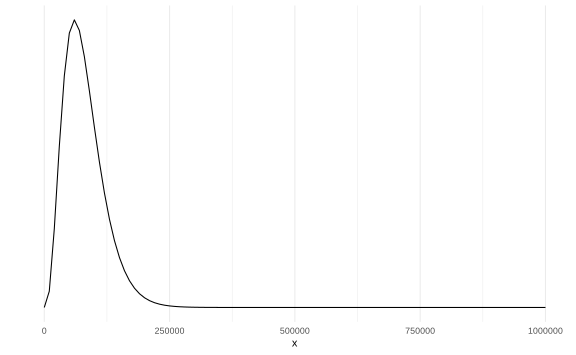
\includegraphics[width=1\linewidth]{Notas-Curso-Estadistica_files/figure-latex/unnamed-chunk-6-1} \end{center}

\hypertarget{distribuciuxf3n-conjunta}{%
\subsection{Distribución conjunta}\label{distribuciuxf3n-conjunta}}

Asumiendo que tenemos algunos datos \(X_1, ..., X_n\), asumimos que estos son exponencial recordando que \(\mathbb E [X] = 1/\theta\), entonces una aproximación de esta densidad es

\begin{Shaded}
\begin{Highlighting}[]
\NormalTok{x \textless{}{-}}\StringTok{ }\KeywordTok{c}\NormalTok{(}\DecValTok{2911}\NormalTok{, }\DecValTok{3403}\NormalTok{, }\DecValTok{3237}\NormalTok{, }\DecValTok{3509}\NormalTok{, }\DecValTok{3118}\NormalTok{)}

\NormalTok{theta \textless{}{-}}\StringTok{ }\DecValTok{1}\OperatorTok{/}\KeywordTok{mean}\NormalTok{(x)}

\KeywordTok{ggplot}\NormalTok{(}\DataTypeTok{data =} \KeywordTok{data.frame}\NormalTok{(}\DataTypeTok{x =} \KeywordTok{c}\NormalTok{(}\DecValTok{0}\NormalTok{, }\FloatTok{1e+05}\NormalTok{)), }\KeywordTok{aes}\NormalTok{(x)) }\OperatorTok{+}\StringTok{ }
\StringTok{    }\KeywordTok{stat\_function}\NormalTok{(}\DataTypeTok{fun =}\NormalTok{ dexp, }\DataTypeTok{args =} \KeywordTok{list}\NormalTok{(}\DataTypeTok{rate =}\NormalTok{ theta)) }\OperatorTok{+}\StringTok{ }
\StringTok{    }\KeywordTok{ylab}\NormalTok{(}\StringTok{""}\NormalTok{) }\OperatorTok{+}\StringTok{ }\KeywordTok{scale\_y\_continuous}\NormalTok{(}\DataTypeTok{breaks =} \OtherTok{NULL}\NormalTok{) }\OperatorTok{+}\StringTok{ }
\StringTok{    }\KeywordTok{theme\_minimal}\NormalTok{()}
\end{Highlighting}
\end{Shaded}

\begin{center}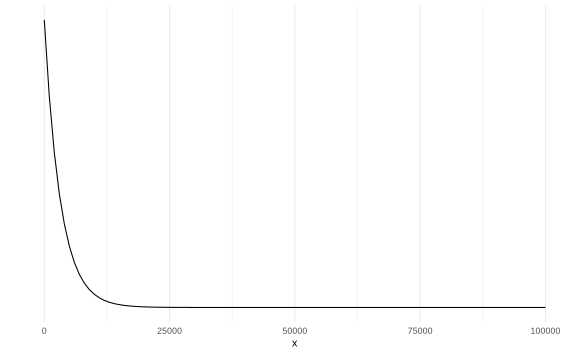
\includegraphics[width=1\linewidth]{Notas-Curso-Estadistica_files/figure-latex/unnamed-chunk-7-1} \end{center}

\hypertarget{distribuciuxf3n-posterior}{%
\subsection{Distribución posterior}\label{distribuciuxf3n-posterior}}

Según los contenidos del curso, se puede estimar los parámetros de la densidad posterior de la forma

\begin{Shaded}
\begin{Highlighting}[]
\NormalTok{(y \textless{}{-}}\StringTok{ }\KeywordTok{sum}\NormalTok{(x))}
\end{Highlighting}
\end{Shaded}

\begin{verbatim}
## [1] 16178
\end{verbatim}

\begin{Shaded}
\begin{Highlighting}[]
\NormalTok{(n \textless{}{-}}\StringTok{ }\KeywordTok{length}\NormalTok{(x))}
\end{Highlighting}
\end{Shaded}

\begin{verbatim}
## [1] 5
\end{verbatim}

\begin{Shaded}
\begin{Highlighting}[]
\NormalTok{(alpha\_posterior \textless{}{-}}\StringTok{ }\NormalTok{n }\OperatorTok{+}\StringTok{ }\NormalTok{alpha\_previa)}
\end{Highlighting}
\end{Shaded}

\begin{verbatim}
## [1] 9
\end{verbatim}

\begin{Shaded}
\begin{Highlighting}[]
\NormalTok{(beta\_posterior \textless{}{-}}\StringTok{ }\NormalTok{beta\_previa }\OperatorTok{+}\StringTok{ }\NormalTok{y)}
\end{Highlighting}
\end{Shaded}

\begin{verbatim}
## [1] 36178
\end{verbatim}

\begin{Shaded}
\begin{Highlighting}[]
\KeywordTok{ggplot}\NormalTok{(}\DataTypeTok{data =} \KeywordTok{data.frame}\NormalTok{(}\DataTypeTok{x =} \KeywordTok{c}\NormalTok{(}\DecValTok{0}\NormalTok{, }\DecValTok{750000}\NormalTok{)), }\KeywordTok{aes}\NormalTok{(x)) }\OperatorTok{+}\StringTok{ }
\StringTok{    }\KeywordTok{stat\_function}\NormalTok{(}\DataTypeTok{fun =}\NormalTok{ dgamma, }\DataTypeTok{args =} \KeywordTok{list}\NormalTok{(}\DataTypeTok{shape =}\NormalTok{ alpha\_previa, }
        \DataTypeTok{scale =}\NormalTok{ beta\_previa), }\KeywordTok{aes}\NormalTok{(}\DataTypeTok{color =} \StringTok{"Previa"}\NormalTok{)) }\OperatorTok{+}\StringTok{ }
\StringTok{    }\KeywordTok{stat\_function}\NormalTok{(}\DataTypeTok{fun =}\NormalTok{ dgamma, }\DataTypeTok{args =} \KeywordTok{list}\NormalTok{(}\DataTypeTok{shape =}\NormalTok{ alpha\_posterior, }
        \DataTypeTok{scale =}\NormalTok{ beta\_posterior), }\KeywordTok{aes}\NormalTok{(}\DataTypeTok{color =} \StringTok{"Posterior"}\NormalTok{)) }\OperatorTok{+}\StringTok{ }
\StringTok{    }\KeywordTok{stat\_function}\NormalTok{(}\DataTypeTok{fun =}\NormalTok{ dexp, }\DataTypeTok{args =} \KeywordTok{list}\NormalTok{(}\DataTypeTok{rate =}\NormalTok{ theta), }
        \KeywordTok{aes}\NormalTok{(}\DataTypeTok{color =} \StringTok{"Verosimilitud"}\NormalTok{)) }\OperatorTok{+}\StringTok{ }\KeywordTok{ylim}\NormalTok{(}\DecValTok{0}\NormalTok{, }\FloatTok{1.5e{-}05}\NormalTok{) }\OperatorTok{+}\StringTok{ }
\StringTok{    }\KeywordTok{theme\_minimal}\NormalTok{()}
\end{Highlighting}
\end{Shaded}

\begin{center}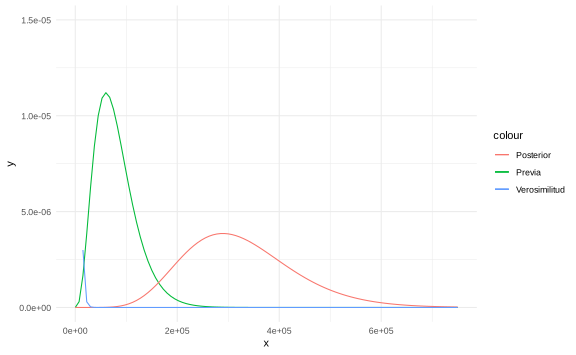
\includegraphics[width=1\linewidth]{Notas-Curso-Estadistica_files/figure-latex/unnamed-chunk-9-1} \end{center}

\hypertarget{agregando-nuevos-datos}{%
\subsection{Agregando nuevos datos}\label{agregando-nuevos-datos}}

Si tenemos un 6to dato, y queremos ver cual es su distribución posterior. Lo primero es estimar la densidad posterior de este 6to dato, pero asumiendo que la previa es la densidad que obtuvimos en el caso anterior.

Suponga que \(X_6 = 3000\)

\begin{Shaded}
\begin{Highlighting}[]
\NormalTok{(alpha\_previa \textless{}{-}}\StringTok{ }\NormalTok{alpha\_posterior)}
\end{Highlighting}
\end{Shaded}

\begin{verbatim}
## [1] 9
\end{verbatim}

\begin{Shaded}
\begin{Highlighting}[]
\NormalTok{(beta\_previa \textless{}{-}}\StringTok{ }\NormalTok{beta\_posterior)}
\end{Highlighting}
\end{Shaded}

\begin{verbatim}
## [1] 36178
\end{verbatim}

\begin{Shaded}
\begin{Highlighting}[]
\NormalTok{(alpha\_posterior \textless{}{-}}\StringTok{ }\NormalTok{alpha\_previa }\OperatorTok{+}\StringTok{ }\DecValTok{1}\NormalTok{)}
\end{Highlighting}
\end{Shaded}

\begin{verbatim}
## [1] 10
\end{verbatim}

\begin{Shaded}
\begin{Highlighting}[]
\NormalTok{(beta\_posterior \textless{}{-}}\StringTok{ }\NormalTok{beta\_previa }\OperatorTok{+}\StringTok{ }\DecValTok{3000}\NormalTok{)}
\end{Highlighting}
\end{Shaded}

\begin{verbatim}
## [1] 39178
\end{verbatim}

\begin{Shaded}
\begin{Highlighting}[]
\KeywordTok{ggplot}\NormalTok{(}\DataTypeTok{data =} \KeywordTok{data.frame}\NormalTok{(}\DataTypeTok{x =} \KeywordTok{c}\NormalTok{(}\DecValTok{0}\NormalTok{, }\FloatTok{1e+06}\NormalTok{)), }\KeywordTok{aes}\NormalTok{(x)) }\OperatorTok{+}\StringTok{ }
\StringTok{    }\KeywordTok{stat\_function}\NormalTok{(}\DataTypeTok{fun =}\NormalTok{ dgamma, }\DataTypeTok{args =} \KeywordTok{list}\NormalTok{(}\DataTypeTok{shape =} \DecValTok{4}\NormalTok{, }
        \DataTypeTok{scale =} \DecValTok{20000}\NormalTok{), }\KeywordTok{aes}\NormalTok{(}\DataTypeTok{color =} \StringTok{"Previa \#1"}\NormalTok{)) }\OperatorTok{+}\StringTok{ }
\StringTok{    }\KeywordTok{stat\_function}\NormalTok{(}\DataTypeTok{fun =}\NormalTok{ dgamma, }\DataTypeTok{args =} \KeywordTok{list}\NormalTok{(}\DataTypeTok{shape =}\NormalTok{ alpha\_previa, }
        \DataTypeTok{scale =}\NormalTok{ beta\_previa), }\KeywordTok{aes}\NormalTok{(}\DataTypeTok{color =} \StringTok{"Previa \#2"}\NormalTok{)) }\OperatorTok{+}\StringTok{ }
\StringTok{    }\KeywordTok{stat\_function}\NormalTok{(}\DataTypeTok{fun =}\NormalTok{ dgamma, }\DataTypeTok{args =} \KeywordTok{list}\NormalTok{(}\DataTypeTok{shape =}\NormalTok{ alpha\_posterior, }
        \DataTypeTok{scale =}\NormalTok{ beta\_posterior), }\KeywordTok{aes}\NormalTok{(}\DataTypeTok{color =} \StringTok{"Posterior"}\NormalTok{)) }\OperatorTok{+}\StringTok{ }
\StringTok{    }\KeywordTok{ylim}\NormalTok{(}\DecValTok{0}\NormalTok{, }\FloatTok{1.5e{-}05}\NormalTok{) }\OperatorTok{+}\StringTok{ }\KeywordTok{theme\_minimal}\NormalTok{()}
\end{Highlighting}
\end{Shaded}

\begin{center}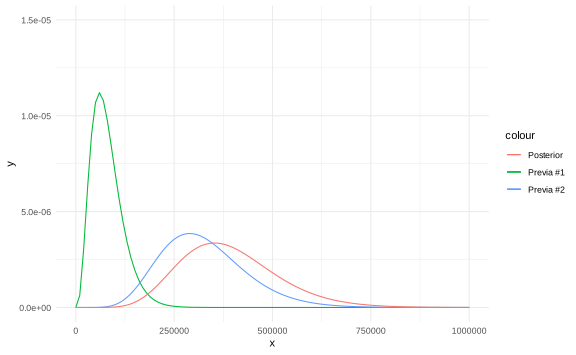
\includegraphics[width=1\linewidth]{Notas-Curso-Estadistica_files/figure-latex/unnamed-chunk-10-1} \end{center}

\hypertarget{familias-conjugadas-normales}{%
\subsection{Familias conjugadas normales}\label{familias-conjugadas-normales}}

Si tenemos pocos datos, la información previa es la que ``prevalece''.

\begin{Shaded}
\begin{Highlighting}[]
\NormalTok{x \textless{}{-}}\StringTok{ }\KeywordTok{rnorm}\NormalTok{(}\DataTypeTok{n =} \DecValTok{3}\NormalTok{, }\DataTypeTok{mean =} \DecValTok{10}\NormalTok{, }\DataTypeTok{sd =} \DecValTok{1}\NormalTok{)}

\NormalTok{(mu \textless{}{-}}\StringTok{ }\KeywordTok{mean}\NormalTok{(x))}
\end{Highlighting}
\end{Shaded}

\begin{verbatim}
## [1] 10.22127
\end{verbatim}

\begin{Shaded}
\begin{Highlighting}[]
\NormalTok{(sigma \textless{}{-}}\StringTok{ }\KeywordTok{sd}\NormalTok{(x))}
\end{Highlighting}
\end{Shaded}

\begin{verbatim}
## [1] 1.185713
\end{verbatim}

\begin{Shaded}
\begin{Highlighting}[]
\NormalTok{(n \textless{}{-}}\StringTok{ }\KeywordTok{length}\NormalTok{(x))}
\end{Highlighting}
\end{Shaded}

\begin{verbatim}
## [1] 3
\end{verbatim}

\begin{Shaded}
\begin{Highlighting}[]
\NormalTok{(mu\_previa \textless{}{-}}\StringTok{ }\DecValTok{0}\NormalTok{)}
\end{Highlighting}
\end{Shaded}

\begin{verbatim}
## [1] 0
\end{verbatim}

\begin{Shaded}
\begin{Highlighting}[]
\NormalTok{(sigma\_previa \textless{}{-}}\StringTok{ }\DecValTok{1}\NormalTok{)}
\end{Highlighting}
\end{Shaded}

\begin{verbatim}
## [1] 1
\end{verbatim}

\begin{Shaded}
\begin{Highlighting}[]
\NormalTok{(mu\_posterior \textless{}{-}}\StringTok{ }\NormalTok{((sigma}\OperatorTok{\^{}}\DecValTok{2}\NormalTok{)}\OperatorTok{/}\NormalTok{(sigma}\OperatorTok{\^{}}\DecValTok{2} \OperatorTok{+}\StringTok{ }\NormalTok{n }\OperatorTok{*}\StringTok{ }\NormalTok{sigma\_previa}\OperatorTok{\^{}}\DecValTok{2}\NormalTok{)) }\OperatorTok{*}\StringTok{ }
\StringTok{    }\NormalTok{mu\_previa }\OperatorTok{+}\StringTok{ }\NormalTok{((n }\OperatorTok{*}\StringTok{ }\NormalTok{sigma\_previa}\OperatorTok{\^{}}\DecValTok{2}\NormalTok{)}\OperatorTok{/}\NormalTok{(sigma}\OperatorTok{\^{}}\DecValTok{2} \OperatorTok{+}\StringTok{ }\NormalTok{n }\OperatorTok{*}\StringTok{ }
\StringTok{    }\NormalTok{sigma\_previa}\OperatorTok{\^{}}\DecValTok{2}\NormalTok{)) }\OperatorTok{*}\StringTok{ }\NormalTok{mu)}
\end{Highlighting}
\end{Shaded}

\begin{verbatim}
## [1] 6.959693
\end{verbatim}

\begin{Shaded}
\begin{Highlighting}[]
\NormalTok{(sigma2\_posterior \textless{}{-}}\StringTok{ }\NormalTok{(sigma}\OperatorTok{\^{}}\DecValTok{2} \OperatorTok{*}\StringTok{ }\NormalTok{sigma\_previa}\OperatorTok{\^{}}\DecValTok{2}\NormalTok{)}\OperatorTok{/}\NormalTok{(sigma}\OperatorTok{\^{}}\DecValTok{2} \OperatorTok{+}\StringTok{ }
\StringTok{    }\NormalTok{n }\OperatorTok{*}\StringTok{ }\NormalTok{sigma\_previa}\OperatorTok{\^{}}\DecValTok{2}\NormalTok{))}
\end{Highlighting}
\end{Shaded}

\begin{verbatim}
## [1] 0.3190971
\end{verbatim}

\begin{Shaded}
\begin{Highlighting}[]
\KeywordTok{ggplot}\NormalTok{(}\DataTypeTok{data =} \KeywordTok{data.frame}\NormalTok{(}\DataTypeTok{x =} \KeywordTok{c}\NormalTok{(}\OperatorTok{{-}}\DecValTok{5}\NormalTok{, }\DecValTok{15}\NormalTok{)), }\KeywordTok{aes}\NormalTok{(x)) }\OperatorTok{+}\StringTok{ }
\StringTok{    }\KeywordTok{stat\_function}\NormalTok{(}\DataTypeTok{fun =}\NormalTok{ dnorm, }\DataTypeTok{args =} \KeywordTok{list}\NormalTok{(}\DataTypeTok{mean =}\NormalTok{ mu\_previa, }
        \DataTypeTok{sd =}\NormalTok{ sigma\_previa), }\KeywordTok{aes}\NormalTok{(}\DataTypeTok{color =} \StringTok{"Previa"}\NormalTok{)) }\OperatorTok{+}\StringTok{ }
\StringTok{    }\KeywordTok{stat\_function}\NormalTok{(}\DataTypeTok{fun =}\NormalTok{ dnorm, }\DataTypeTok{args =} \KeywordTok{list}\NormalTok{(}\DataTypeTok{mean =}\NormalTok{ mu\_posterior, }
        \DataTypeTok{sd =} \KeywordTok{sqrt}\NormalTok{(sigma2\_posterior)), }\KeywordTok{aes}\NormalTok{(}\DataTypeTok{color =} \StringTok{"Posterior"}\NormalTok{)) }\OperatorTok{+}\StringTok{ }
\StringTok{    }\KeywordTok{stat\_function}\NormalTok{(}\DataTypeTok{fun =}\NormalTok{ dnorm, }\DataTypeTok{args =} \KeywordTok{list}\NormalTok{(}\DataTypeTok{mean =}\NormalTok{ mu, }
        \DataTypeTok{sd =}\NormalTok{ sigma), }\KeywordTok{aes}\NormalTok{(}\DataTypeTok{color =} \StringTok{"Verosimilitud"}\NormalTok{)) }\OperatorTok{+}\StringTok{ }
\StringTok{    }\KeywordTok{theme\_minimal}\NormalTok{()}
\end{Highlighting}
\end{Shaded}

\begin{center}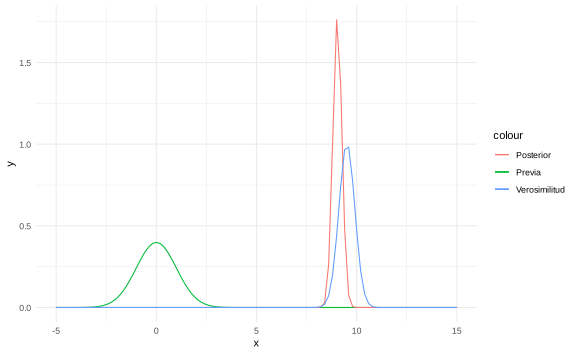
\includegraphics[width=1\linewidth]{Notas-Curso-Estadistica_files/figure-latex/unnamed-chunk-11-1} \end{center}

Con más datos, la distribución se ajusta a esto y le quita importancia a la información previa.

\begin{Shaded}
\begin{Highlighting}[]
\NormalTok{x \textless{}{-}}\StringTok{ }\KeywordTok{rnorm}\NormalTok{(}\DataTypeTok{n =} \DecValTok{100}\NormalTok{, }\DataTypeTok{mean =} \DecValTok{10}\NormalTok{, }\DataTypeTok{sd =} \DecValTok{1}\NormalTok{)}

\NormalTok{(mu \textless{}{-}}\StringTok{ }\KeywordTok{mean}\NormalTok{(x))}
\end{Highlighting}
\end{Shaded}

\begin{verbatim}
## [1] 9.890422
\end{verbatim}

\begin{Shaded}
\begin{Highlighting}[]
\NormalTok{(sigma \textless{}{-}}\StringTok{ }\KeywordTok{sd}\NormalTok{(x))}
\end{Highlighting}
\end{Shaded}

\begin{verbatim}
## [1] 1.134588
\end{verbatim}

\begin{Shaded}
\begin{Highlighting}[]
\NormalTok{(n \textless{}{-}}\StringTok{ }\KeywordTok{length}\NormalTok{(x))}
\end{Highlighting}
\end{Shaded}

\begin{verbatim}
## [1] 100
\end{verbatim}

\begin{Shaded}
\begin{Highlighting}[]
\NormalTok{(mu\_previa \textless{}{-}}\StringTok{ }\DecValTok{0}\NormalTok{)}
\end{Highlighting}
\end{Shaded}

\begin{verbatim}
## [1] 0
\end{verbatim}

\begin{Shaded}
\begin{Highlighting}[]
\NormalTok{(sigma\_previa \textless{}{-}}\StringTok{ }\DecValTok{1}\NormalTok{)}
\end{Highlighting}
\end{Shaded}

\begin{verbatim}
## [1] 1
\end{verbatim}

\begin{Shaded}
\begin{Highlighting}[]
\NormalTok{(mu\_posterior \textless{}{-}}\StringTok{ }\NormalTok{((sigma}\OperatorTok{\^{}}\DecValTok{2}\NormalTok{)}\OperatorTok{/}\NormalTok{(sigma}\OperatorTok{\^{}}\DecValTok{2} \OperatorTok{+}\StringTok{ }\NormalTok{n }\OperatorTok{*}\StringTok{ }\NormalTok{sigma\_previa}\OperatorTok{\^{}}\DecValTok{2}\NormalTok{)) }\OperatorTok{*}\StringTok{ }
\StringTok{    }\NormalTok{mu\_previa }\OperatorTok{+}\StringTok{ }\NormalTok{((n }\OperatorTok{*}\StringTok{ }\NormalTok{sigma\_previa}\OperatorTok{\^{}}\DecValTok{2}\NormalTok{)}\OperatorTok{/}\NormalTok{(sigma}\OperatorTok{\^{}}\DecValTok{2} \OperatorTok{+}\StringTok{ }\NormalTok{n }\OperatorTok{*}\StringTok{ }
\StringTok{    }\NormalTok{sigma\_previa}\OperatorTok{\^{}}\DecValTok{2}\NormalTok{)) }\OperatorTok{*}\StringTok{ }\NormalTok{mu)}
\end{Highlighting}
\end{Shaded}

\begin{verbatim}
## [1] 9.764722
\end{verbatim}

\begin{Shaded}
\begin{Highlighting}[]
\NormalTok{(sigma2\_posterior \textless{}{-}}\StringTok{ }\NormalTok{(sigma}\OperatorTok{\^{}}\DecValTok{2} \OperatorTok{*}\StringTok{ }\NormalTok{sigma\_previa}\OperatorTok{\^{}}\DecValTok{2}\NormalTok{)}\OperatorTok{/}\NormalTok{(sigma}\OperatorTok{\^{}}\DecValTok{2} \OperatorTok{+}\StringTok{ }
\StringTok{    }\NormalTok{n }\OperatorTok{*}\StringTok{ }\NormalTok{sigma\_previa}\OperatorTok{\^{}}\DecValTok{2}\NormalTok{))}
\end{Highlighting}
\end{Shaded}

\begin{verbatim}
## [1] 0.01270929
\end{verbatim}

\begin{Shaded}
\begin{Highlighting}[]
\KeywordTok{ggplot}\NormalTok{(}\DataTypeTok{data =} \KeywordTok{data.frame}\NormalTok{(}\DataTypeTok{x =} \KeywordTok{c}\NormalTok{(}\OperatorTok{{-}}\DecValTok{5}\NormalTok{, }\DecValTok{15}\NormalTok{)), }\KeywordTok{aes}\NormalTok{(x)) }\OperatorTok{+}\StringTok{ }
\StringTok{    }\KeywordTok{stat\_function}\NormalTok{(}\DataTypeTok{fun =}\NormalTok{ dnorm, }\DataTypeTok{args =} \KeywordTok{list}\NormalTok{(}\DataTypeTok{mean =}\NormalTok{ mu\_previa, }
        \DataTypeTok{sd =}\NormalTok{ sigma\_previa), }\KeywordTok{aes}\NormalTok{(}\DataTypeTok{color =} \StringTok{"Previa"}\NormalTok{)) }\OperatorTok{+}\StringTok{ }
\StringTok{    }\KeywordTok{stat\_function}\NormalTok{(}\DataTypeTok{fun =}\NormalTok{ dnorm, }\DataTypeTok{args =} \KeywordTok{list}\NormalTok{(}\DataTypeTok{mean =}\NormalTok{ mu\_posterior, }
        \DataTypeTok{sd =} \KeywordTok{sqrt}\NormalTok{(sigma2\_posterior)), }\KeywordTok{aes}\NormalTok{(}\DataTypeTok{color =} \StringTok{"Posterior"}\NormalTok{)) }\OperatorTok{+}\StringTok{ }
\StringTok{    }\KeywordTok{stat\_function}\NormalTok{(}\DataTypeTok{fun =}\NormalTok{ dnorm, }\DataTypeTok{args =} \KeywordTok{list}\NormalTok{(}\DataTypeTok{mean =}\NormalTok{ mu, }
        \DataTypeTok{sd =}\NormalTok{ sigma), }\KeywordTok{aes}\NormalTok{(}\DataTypeTok{color =} \StringTok{"Verosimilitud"}\NormalTok{)) }\OperatorTok{+}\StringTok{ }
\StringTok{    }\KeywordTok{theme\_minimal}\NormalTok{()}
\end{Highlighting}
\end{Shaded}

\begin{center}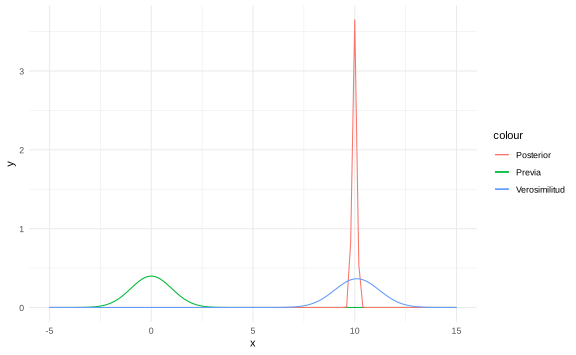
\includegraphics[width=1\linewidth]{Notas-Curso-Estadistica_files/figure-latex/unnamed-chunk-12-1} \end{center}

Si los datos por si solo son muy variable, la posterior tiende a parecerse a la
distribución previa en lugar que a la verosimilitud.

\begin{Shaded}
\begin{Highlighting}[]
\NormalTok{x \textless{}{-}}\StringTok{ }\KeywordTok{rnorm}\NormalTok{(}\DataTypeTok{n =} \DecValTok{10}\NormalTok{, }\DataTypeTok{mean =} \DecValTok{10}\NormalTok{, }\DataTypeTok{sd =} \DecValTok{5}\NormalTok{)}

\NormalTok{(mu \textless{}{-}}\StringTok{ }\KeywordTok{mean}\NormalTok{(x))}
\end{Highlighting}
\end{Shaded}

\begin{verbatim}
## [1] 10.90214
\end{verbatim}

\begin{Shaded}
\begin{Highlighting}[]
\NormalTok{(sigma \textless{}{-}}\StringTok{ }\KeywordTok{sd}\NormalTok{(x))}
\end{Highlighting}
\end{Shaded}

\begin{verbatim}
## [1] 5.107251
\end{verbatim}

\begin{Shaded}
\begin{Highlighting}[]
\NormalTok{(n \textless{}{-}}\StringTok{ }\KeywordTok{length}\NormalTok{(x))}
\end{Highlighting}
\end{Shaded}

\begin{verbatim}
## [1] 10
\end{verbatim}

\begin{Shaded}
\begin{Highlighting}[]
\NormalTok{(mu\_previa \textless{}{-}}\StringTok{ }\DecValTok{0}\NormalTok{)}
\end{Highlighting}
\end{Shaded}

\begin{verbatim}
## [1] 0
\end{verbatim}

\begin{Shaded}
\begin{Highlighting}[]
\NormalTok{(sigma\_previa \textless{}{-}}\StringTok{ }\DecValTok{1}\NormalTok{)}
\end{Highlighting}
\end{Shaded}

\begin{verbatim}
## [1] 1
\end{verbatim}

\begin{Shaded}
\begin{Highlighting}[]
\NormalTok{(mu\_posterior \textless{}{-}}\StringTok{ }\NormalTok{((sigma}\OperatorTok{\^{}}\DecValTok{2}\NormalTok{)}\OperatorTok{/}\NormalTok{(sigma}\OperatorTok{\^{}}\DecValTok{2} \OperatorTok{+}\StringTok{ }\NormalTok{n }\OperatorTok{*}\StringTok{ }\NormalTok{sigma\_previa}\OperatorTok{\^{}}\DecValTok{2}\NormalTok{)) }\OperatorTok{*}\StringTok{ }
\StringTok{    }\NormalTok{mu\_previa }\OperatorTok{+}\StringTok{ }\NormalTok{((n }\OperatorTok{*}\StringTok{ }\NormalTok{sigma\_previa}\OperatorTok{\^{}}\DecValTok{2}\NormalTok{)}\OperatorTok{/}\NormalTok{(sigma}\OperatorTok{\^{}}\DecValTok{2} \OperatorTok{+}\StringTok{ }\NormalTok{n }\OperatorTok{*}\StringTok{ }
\StringTok{    }\NormalTok{sigma\_previa}\OperatorTok{\^{}}\DecValTok{2}\NormalTok{)) }\OperatorTok{*}\StringTok{ }\NormalTok{mu)}
\end{Highlighting}
\end{Shaded}

\begin{verbatim}
## [1] 3.021321
\end{verbatim}

\begin{Shaded}
\begin{Highlighting}[]
\NormalTok{(sigma2\_posterior \textless{}{-}}\StringTok{ }\NormalTok{(sigma}\OperatorTok{\^{}}\DecValTok{2} \OperatorTok{*}\StringTok{ }\NormalTok{sigma\_previa}\OperatorTok{\^{}}\DecValTok{2}\NormalTok{)}\OperatorTok{/}\NormalTok{(sigma}\OperatorTok{\^{}}\DecValTok{2} \OperatorTok{+}\StringTok{ }
\StringTok{    }\NormalTok{n }\OperatorTok{*}\StringTok{ }\NormalTok{sigma\_previa}\OperatorTok{\^{}}\DecValTok{2}\NormalTok{))}
\end{Highlighting}
\end{Shaded}

\begin{verbatim}
## [1] 0.722869
\end{verbatim}

\begin{Shaded}
\begin{Highlighting}[]
\KeywordTok{ggplot}\NormalTok{(}\DataTypeTok{data =} \KeywordTok{data.frame}\NormalTok{(}\DataTypeTok{x =} \KeywordTok{c}\NormalTok{(}\OperatorTok{{-}}\DecValTok{5}\NormalTok{, }\DecValTok{15}\NormalTok{)), }\KeywordTok{aes}\NormalTok{(x)) }\OperatorTok{+}\StringTok{ }
\StringTok{    }\KeywordTok{stat\_function}\NormalTok{(}\DataTypeTok{fun =}\NormalTok{ dnorm, }\DataTypeTok{args =} \KeywordTok{list}\NormalTok{(}\DataTypeTok{mean =}\NormalTok{ mu\_previa, }
        \DataTypeTok{sd =}\NormalTok{ sigma\_previa), }\KeywordTok{aes}\NormalTok{(}\DataTypeTok{color =} \StringTok{"Previa"}\NormalTok{)) }\OperatorTok{+}\StringTok{ }
\StringTok{    }\KeywordTok{stat\_function}\NormalTok{(}\DataTypeTok{fun =}\NormalTok{ dnorm, }\DataTypeTok{args =} \KeywordTok{list}\NormalTok{(}\DataTypeTok{mean =}\NormalTok{ mu\_posterior, }
        \DataTypeTok{sd =} \KeywordTok{sqrt}\NormalTok{(sigma2\_posterior)), }\KeywordTok{aes}\NormalTok{(}\DataTypeTok{color =} \StringTok{"Posterior"}\NormalTok{)) }\OperatorTok{+}\StringTok{ }
\StringTok{    }\KeywordTok{stat\_function}\NormalTok{(}\DataTypeTok{fun =}\NormalTok{ dnorm, }\DataTypeTok{args =} \KeywordTok{list}\NormalTok{(}\DataTypeTok{mean =}\NormalTok{ mu, }
        \DataTypeTok{sd =}\NormalTok{ sigma), }\KeywordTok{aes}\NormalTok{(}\DataTypeTok{color =} \StringTok{"Verosimilitud"}\NormalTok{)) }\OperatorTok{+}\StringTok{ }
\StringTok{    }\KeywordTok{theme\_minimal}\NormalTok{()}
\end{Highlighting}
\end{Shaded}

\begin{center}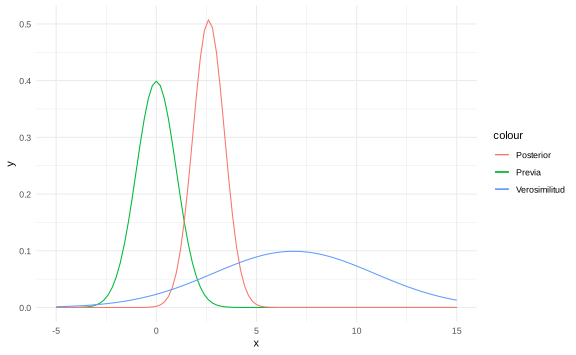
\includegraphics[width=1\linewidth]{Notas-Curso-Estadistica_files/figure-latex/unnamed-chunk-13-1} \end{center}

\hypertarget{funciones-de-puxe9rdida-1}{%
\subsection{Funciones de pérdida}\label{funciones-de-puxe9rdida-1}}

Lo más importante acá es que dependiendo de la función de pérdida podemos construir una estimador para \(\theta\). En el caso de los componentes electrónicos recordemos que la posterior nos daba

\begin{Shaded}
\begin{Highlighting}[]
\NormalTok{alpha \textless{}{-}}\StringTok{ }\DecValTok{9}
\NormalTok{beta \textless{}{-}}\StringTok{ }\DecValTok{36178}
\end{Highlighting}
\end{Shaded}

\begin{itemize}
\tightlist
\item
  \textbf{Pérdida cuadrática:} Recoremos que la media de una gamma es \(\alpha/\beta\) entonces
\end{itemize}

\begin{Shaded}
\begin{Highlighting}[]
\NormalTok{(theta \textless{}{-}}\StringTok{ }\NormalTok{alpha}\OperatorTok{/}\NormalTok{beta)}
\end{Highlighting}
\end{Shaded}

\begin{verbatim}
## [1] 0.00024877
\end{verbatim}

Y por lo tanto el tiempo promedio del componente electrónico es \(1/\theta\)=4019.7777778.

\begin{itemize}
\tightlist
\item
  \textbf{Pérdidad absoluta:} La distribución Gamma no tiene una forma cerrada para la mediana, por que se puede aproximar así,
\end{itemize}

\begin{Shaded}
\begin{Highlighting}[]
\NormalTok{m \textless{}{-}}\StringTok{ }\KeywordTok{rgamma}\NormalTok{(}\DataTypeTok{n =} \DecValTok{1000}\NormalTok{, }\DataTypeTok{scale =}\NormalTok{ beta, }\DataTypeTok{shape =}\NormalTok{ alpha)}
\NormalTok{(theta \textless{}{-}}\StringTok{ }\KeywordTok{median}\NormalTok{(m))}
\end{Highlighting}
\end{Shaded}

\begin{verbatim}
## [1] 317434.4
\end{verbatim}

Y por lo tanto el tiempo promedio del componente electrónico es \(1/\theta\)=\ensuremath{3.1502569\times 10^{-6}}.

\textbf{OJO: En este caso la pérdida cuadrática ajusta mejor ya que la distribución que la pérdida absoluta ya que la distribución NO es simétrica. En el caso simétrico los resultados serían muy similares.}

\hypertarget{estimaciuxf3n-por-muxe1xima-verosimilitud}{%
\chapter{Estimación por máxima verosimilitud}\label{estimaciuxf3n-por-muxe1xima-verosimilitud}}

¿Será posible estimar sin una densidad previa? Se debería ajustar la noción de muestra a independencia dado el valor de un parámetro.

Recuerde que, para \(X_1,\dots, X_n \stackrel{i.i.d}{\sim} f(X|\theta)\) con \(\theta\) fijo, la \textbf{función de verosimilitud} se define como
\[ f_n(X|\theta) = \pi(X_i|\theta) = G(\theta|X).\]

Si \(\theta_1,\theta_2\in \Omega\), \(\theta\) es el valor real del parámetro. Si la muestra es fija, evaluamos, para \(\theta_1\), \(f_n(X|\theta_1) = G(\theta_1|X)\) y, de igual forma para \(\theta_2\), \(f_n(X|\theta_2) = G(\theta_2|X)\). Supongamos que
\[f_n(X|\theta_1) >f_n(X|\theta_2) \implies G(\theta_1|X)>G(\theta_2|X) \text{ (principio de verosimilitud)}\]

\textbf{Interpretación}. Es más verosímil (realista) que el verdadero parámetro sea \(\theta_1\) que \(\theta_2\) dada la muestra.

\textbf{Definición}. Para cada \(x\in \mathcal{X}\) (espacio muestral), sea \(\delta(x) \in \delta\) estimador de \(\theta\) tal que \(f_n(x|\theta)\) es máximo. A \(\delta(x)\) se le llama \textbf{MLE (estimador de máxima verosimilitud)}.

\textbf{Ejemplo}. Si \(X_1,\dots, X_n \sim \text{Exp}(\theta)\), estime \(\theta\).

Determinamos la función de verosimilitud,
\[f_n(X|\theta) = \prod_{i=1}^n \dfrac{1}\theta e^{-X_i/\theta} = \dfrac1{\theta^n} \exp\left(\dfrac{1}\theta \sum_{i=1}^nX_i\right) = \theta^{-n}e^{-y/\theta}.\]

Considere la \textbf{log-verosimilitud}

\[L(\theta|X) = \ln f_n(X|\theta) = -n\ln \theta - \dfrac{y}{\theta}\]

Como es una transformación monótona creciente, la función de verosimilitud se maximiza si la log-verosimilitud es máxima. Entonces,

\[\dfrac{\partial}{\partial\theta} L(\theta|X) = \dfrac{-n}{\theta}+\dfrac{y}{\theta^2} = 0\implies \dfrac{1}{\theta}\left(-n+\dfrac{y}\theta\right)=0 \implies \hat\theta = \dfrac{y}{n} = \bar X_n.\]
Para verificar que es un máximo:

\[\dfrac{\partial^2 L}{\partial\theta^2} = \left. \dfrac{n}{\theta^2} -\dfrac{2y}{\theta^3}\right\vert_{\theta = \frac{y}{n}} = \dfrac{1}{\hat\theta^2} \bigg[n-\dfrac{2y}{\frac yn}\bigg] = \dfrac{-n}{\hat\theta^2} < 0.\]

Entonces \(\hat\theta = \bar X_n\) es el MLE de \(\theta\).

\textbf{Ejemplo}. En una prueba sobre alguna enfermedad, en un \(90\%\) da la verdadera condición (enfermo) y en un \(10\%\) la prueba se equivoca (que diga que la persona esté enferma cuando está sana). Considere una variable aleatoria \(\text{Bernoulli}(\theta)\),\(\theta \in \{0.9,0.1\}\)
Una muestra sería
\[x = \begin{cases}1 & \text{si la prueba es positiva}\\0& \text{si no}\end{cases}\]
Si \(x=0\), entonces \(f(0|\theta) = \begin{cases}0.9 & \text{si }\theta = 0.1\\0.1& \text{si }\theta = 0.9\end{cases}\).

Si \(x=1\), entonces \(f(1|\theta) = \begin{cases}0.1 & \text{si }\theta = 0.1\\0.9& \text{si }\theta = 0.9\end{cases}\).

El MLE corresponde a
\[\hat\theta = \begin{cases}0.1 & \text{si }x= 0\\0.9& \text{si }x= 1\end{cases}\]
\textbf{Ejemplo}. Para el caso normal, \(X_1,\dots, X_n \sim N(\mu,\sigma^2)\), \(\sigma^2\) conocida, estime \(\mu\).

\[f_n(x|\mu) = \prod_{i=1}^n \dfrac{1}{\sqrt{2\pi\sigma^2}}\exp\left(-\dfrac{(x_i-\mu)^2}{2\sigma^2}\right) = (2\pi\sigma^2)^{-n/2}\exp\left(-\dfrac1{2\sigma^2}\sum_{i=1}^n(x_i-\mu)^2\right).\]

La log-verosimilitud es de la forma
\[ L(\mu|x) = \dfrac{-n}{2}\ln(2\pi\sigma^2)-\dfrac1{2\sigma^2}\sum_{i=1}^n(x_i-\mu)^2.\]

Basta con minimizar \(Q(\mu) = \sum_{i=1}^n(x_i-\mu)^2\).

\[ \dfrac{\partial Q}{\partial\mu} = -2\sum_{i=1}^n(x_i-\mu) \implies n\mu = \sum_{i=1}^nx_i \implies \hat\mu = \bar x_n.\]

No hace falta verificar la condición de segundo orden, pues \(Q\) es una función cuadrática de \(\mu\) y tiene un único máximo.

\[ \hat\mu_{MLE} = \bar x_n \quad (*)\]

Ahora, si \(X_1,\dots, X_n \sim N(\mu,\sigma^2)\), \(\theta = (\mu,\sigma^2)\) desconocido, por \((*)\),
\[ L(\sigma^2|X_1,\dots, X_n) = \dfrac n2 \ln(2\pi\sigma^2)--\dfrac1{2\sigma^2}\sum_{i=1}^n(x_i-\bar x_n)^2\]

\[ \dfrac{\partial L}{\partial\sigma^2} = -\dfrac n2 \dfrac1{2\pi\sigma^2} + \dfrac1{2(\sigma^2)^2} \sum_{i=1}^n(x_i-\bar x_n)^2= 0 \]
Entonces
\[ \sigma^2 = \dfrac 1n \sum_{i=1}^n(x_i-\mu)^2 \text{ (varianza muestral)}\]

Las condiciones de segundo orden quedan como ejercicio.

\textbf{Nota}. Si \(\theta_{MLE}\) de \(\theta\), entonces \(h(\theta_{MLE})\) es el MLE de \(h(\theta)\).

Sea \(h(x,y) = \sqrt{y}\) (es inyectiva). \(h(\bar x_n, \hat\sigma^2) = \sqrt{\hat\sigma^2} = \hat\sigma\).

El MLE de \(\dfrac{\sigma}{\mu} = \dfrac{\hat \sigma}{\bar x_n}\).

\textbf{Ejemplo}. \(X_1,\dots, X_n \stackrel{i.i.d}{\sim} \text{Unif}(0)\). Estime \(\theta\) \((\theta > 0)\). Suponga que \(x_i>0 \forall i\).

\[f(X|\theta) = \dfrac 1\theta \cdot 1_{[0,\theta]}(x)\]

La verosimilitud es
\[f_n(x|\theta) = \prod_{i=1}^{n} f(x_i|\theta) = \dfrac 1{\theta^n} \prod_{i=1}^n 1_{\{0\leq x_i\leq \theta\}} \quad 0\leq x_i \leq \theta \;\forall i\]
Vea que \(f_n(x|\theta)\) es positivo si y solo si \(O\leq X_{(n)}\leq \theta\).

El valor de la muestra \(\{X_1,\dots, X_n\}\) en la \(i\)-ésima posición cuando los datos se ordenan de menor a mayor se denota \(X_{(i)}\) (estadístico de orden). En este caso, \(X_{(n)} = \max\{X_1,\dots, X_n\}\).
Entonces \(\hat\theta_{MLE} = x_{(n)}\).

\hypertarget{propiedades-del-mle}{%
\chapter{Propiedades del MLE}\label{propiedades-del-mle}}

\hypertarget{propiedad-de-invarianza}{%
\section{Propiedad de invarianza}\label{propiedad-de-invarianza}}

\textbf{Teorema}. Si \(\hat\theta\) es el MLE de \(\hat\theta\) y si \(g\) es biyectiva, entonces \(g(\theta)\) es el MLE de \(g(\theta)\).

\emph{Prueba}:

Sea \(\Gamma\) el espacio paramétrico \(g(\Omega)\). Como \(g\) es biyectiva entonces \(h:\) inversa de \(g\): \(\theta = h(\psi), \psi \in \Gamma\).

Reparametrizando la verosimilitud,
\[f_n(x|\theta) = f_n(x|h(\psi)). \]

El MLE de \(\psi:\hat\psi\) satisface que \(f_n(x|h(\hat\psi))\) es máximo.

Como \(f_n(x|\theta)\) se maximiza cuando \(\theta = \hat \theta\), entonces \(f_n(x|h(\psi))\) se maximiza cuando \(\hat \theta = h(\psi)\) para algún \(\psi\).

Se concluye que \(\hat\theta = h(\hat\psi) \implies \hat\psi = g(\hat \theta)\).

\textbf{Ejemplo}: \(g(\theta) = \dfrac 1\theta\) es biyectiva si \(\theta > 0\). Así,

\[ \hat{\dfrac 1 \theta} = \dfrac 1{\hat \theta} = \dfrac{1}{\frac 1{\hat X_n}} = \hat X_n \quad(\theta \text{ es parámetro de tasa}).\]
¿Qué pasa si \(h\) no es biyectiva?

\textbf{Definicion (Generalización del MLE)}. Si \(g\) es una función de \(\theta\) y \(G\) la imagen de \(\Omega\) bajo \(g\). Para cada \(t\in G\) defina
\[ G_t = \{\theta: g(\theta) = t\}\]
Defina \(L^*(t) = \displaystyle\max_{\theta\in G_t} \ln f_n(x|\theta)\). El MLE de \(g(\theta) (=\hat t)\) satisface \(L^*(\hat t) = \displaystyle\max_{t \in G} L^*(t)\).

\textbf{Teorema}. Si \(\hat \theta\) es el MLE de \(\theta\) entonces \(g(\hat\theta)\) es el MLE de \(g(\theta)\) (\(g\) es arbitraria).

\emph{Prueba}. Basta probar \(L^*(\hat t) = \ln f_n(x|\hat \theta)\). Se cumple que \(\hat\theta\in G_{\hat t}\). Como \(\hat \theta\) maximiza \(f_n(x|\theta)\) \(\forall \theta\), también lo hace si \(\theta \in G_{\hat t}\). Entonces \(\hat t = g(\hat \theta)\) (no pueden existir 2 máximos en un conjunto con la misma imagen).

\textbf{Ejemplos}.\(X_1,\dots, X_n \sim N(\mu, \sigma^2)\).

\begin{itemize}
\item
  Si \(h(\mu, \sigma^2) = \sigma\) (no es biyectiva) \(\implies h(\hat X_n,\hat\sigma^2) = \sqrt{\hat\sigma^2}\) es el MLE de \(\sigma\).
\item
  \(h(\mu,\sigma^2) = \dfrac{\sigma^*}{\mu}\) (coeficiente de variación). \(\dfrac{\hat{\sigma}}{\bar X_n}\) es el MLE de CV.
\item
  \(h(\mu, \sigma^2) = \mu^2 + \sigma^2\). \(\mathbb{E}[X^2] - \mu^2 = \sigma^2 \implies \mathbb{E}[X^2] = \mu^2 + \sigma^2\). El MLE de \(\mathbb{E}[X^2]\) es \(\bar X_n^2 + \hat \sigma ^2\).
\end{itemize}

\hypertarget{consistencia}{%
\section{Consistencia}\label{consistencia}}

Los estimadores bayesianos son de la forma
\[EB = W_1\mathbb{E}[\text{Previa}] + W_2\hat X_n.\]
El estimador bayesiano ``combina'' la esperanza de la previa y el \(\hat\theta_{MLE}\). El \(\hat\theta_{MLE}\) ``hereda la consistencia del estimador bayesiano''.

\[EB = W_1\mathbb{E}[\text{Previa}] + W_2 \hat\theta_{MLE}.\]
\textbf{Afirmación}. Bajo ``condiciones usuales'',
\[\hat\theta_{MLE} \xrightarrow[n\to \infty]{\mathbb P}\theta.\]

\hypertarget{cuxe1lculo-numuxe9rico}{%
\chapter{Cálculo numérico}\label{cuxe1lculo-numuxe9rico}}

\hypertarget{muxe9todo-de-los-momentos}{%
\section{Método de los momentos}\label{muxe9todo-de-los-momentos}}

\textbf{Ejemplo}. \(X_1,\dots, X_n \sim \Gamma(\alpha,1)\). Estime \(\alpha\).
\[f_n(x|\alpha) = \dfrac{1}{\Gamma(\alpha)}x^{\alpha-1}e^{-x}.\]

Verosimilitud: \(f_n(x|\alpha) = \dfrac 1 {\Gamma(\alpha)^n}(\prod x_i)e^{\sum x_i}\).

\begin{align*}
\dfrac{\partial}{\partial \alpha} L(\alpha|x) & = \dfrac{\partial}{\partial \alpha} \bigg[ -n\ln \Gamma(\alpha) + (\alpha-1)\ln(\pi x_i) - \sum x_i\bigg]\\
& = -n\dfrac{1}{\Gamma(\alpha)} \dfrac d{d\alpha}\Gamma(\alpha) + \ln (\prod x_i) = 0
\end{align*}

\textbf{Definición}. Asumimos que \(X_1,\dots, X_n \sim F\) indexada con un parámetro \(\theta \in \mathbb{R}^k\) y que al menos tiene \(k\) momentos finitos. Para \(j = 1,\dots, k\) sea \(\mu_j(\theta) = \mathbb{E}[X_1^j|\theta]\). Suponga que \(\mu(\theta) = (\mu_1(\theta),\dots,\mu_2(\theta))\) es biyectiva. Sea \(M\) la inversa de \(\mu\),
\[ M(\mu(\theta)) = \theta =M(\mu_1(\theta),\dots,\mu_2(\theta)) \]
y defina los momentos empíricos
\[ m_j = \dfrac 1n \sum_{i=1}^n X_i^j, \quad j=1,\dots, k.\]
El estimador según el método de los momentos es
\[\hat\theta = M(m_1,\dots,m_k).\]
Del ejemplo anterior, \(\mu_1(\alpha) = \mathbb{E}[x_1|\alpha] = \alpha\).Dado que \(m_1 = \hat x_n\), el sistema por resolver es
\[ \mu_1(\alpha) = m_1 \Longleftrightarrow \alpha = \bar x_n\]
El estimador por método de momentos es \(\hat \alpha = \bar X_n\).

\textbf{Ejemplo}. \(X_1,\dots, X_n \stackrel{i.i.d}{\sim} \Gamma(\alpha, \beta)\). La varianza de \(X\) es
\[ \dfrac{\alpha}{\beta^2} = \text{Var}X = \mathbb{E}[X^2]-\mathbb{E}[X]^2 = \mathbb{E}[X^2] - \dfrac{\alpha^2}{\beta^2}.\]
Se debe resolver el sistema
\[ \begin{cases}\mu_1(\theta) = \dfrac{\alpha}\beta = \bar X_n = m_1& (1)\\\mu_2(\theta) = \dfrac{\alpha(\alpha+1)}{\beta^2}=m_2 & (2)\end{cases}\]

De \((1)\), \(\alpha = m_1\beta\). Sustituyendo en \((2)\),

\[m_2 = \dfrac{m_1\beta(m_1\beta+1)}{\beta^2} = m_1^2+\dfrac{m_1}\beta = m_2\implies m_2-m_1^2 = \dfrac{m_1}{\beta}.\]
De esta manera,
\[ \hat\beta = \dfrac{m_1}{m_2-m_1^2},\quad  \hat\alpha = \dfrac{m_1^2}{m_2-m_1^2}\]
\textbf{Teorema}. Si \(X_1,X_2,\dots\) i.i.d con distribución indexada por \(\theta \in \mathbb{R}^k\). Suponga que los \(k\) momoentos teóricos son finitos \(\forall \theta\) y suponga que \(M\) es continua. Entonces el estimador por el método de momentos es consistente.

¿Cuál es el comportamiento en la distribución de \(\hat\theta\) cuando la muestra es grande?

Del teorema del límite central,
\[ \dfrac{\bar X_n-\theta}{\dfrac{\sigma}{\sqrt{n}}} = \dfrac{\sqrt{n}(\bar X_n-\theta)}{\sigma} \xrightarrow{d} N(0,1)\]
\[\text{Var}(\bar X_n) = \dfrac 1{n^2}\sum \text{Var}(X_1) = \dfrac{\sigma^2}n\]

Implica que se debe multiplicar la media muestral por una constante para hacer la desviación visibile y, con ello, hacer inferencia del parámetro.

\textbf{Caso general}. Si \(f(X|\theta)\) es ``suficientemente suave'' como función de \(\theta\), es puede comprobar que la verosimilitud tiende a una normal conforme \(n \to \infty\). Es decir,
\[ f(X|\theta)\propto \exp\Bigg[\dfrac{-1}{2\frac{V_n(\theta)}{n}}(\theta-\hat\theta)\Bigg], \quad n \to \infty\quad(*) \]
donde \(\hat\theta\) es el MLE de \(\theta\).

\[V_n(\theta)\xrightarrow[n\to \infty]{}V_{\infty}(\theta)<\infty\]

\textbf{Notas}:

\begin{enumerate}
\def\labelenumi{\arabic{enumi})}
\item
  Si \(n \to \infty\) la normal en \((*)\) tiene muchísima precisión y es concentrada alrededor de \(\hat\theta\).
\item
  En el caso bayesiano, ninguna previa en \(\theta\) puede anular el efecto en la verosimilitud cuando \(n\to \infty\).
\item
  Por \((*)\) el MLE se distribute asintóticamente como \[N\left(\theta, \dfrac{V_\infty(\theta)}{n}\right),\] \(Var(X_n)\xrightarrow[n\to \infty]{} 0\) y \(\mathbb{E}[X_n] = X \implies X_n \xrightarrow[n\to \infty]{\mathbb P} X\) (confirma que el MLE es consistente).
\end{enumerate}

\hypertarget{muxe9todo-delta}{%
\section{Método Delta}\label{muxe9todo-delta}}

Si \(Y_1,Y_2,\dots\) es una sucesión de variables aleatorias y sea \(F^*\) su c.d.f. continua. Sea \(\theta\in \mathbb R\) y \(\{a_n\}\) sucesión de números positivos tal que \(a_n \nearrow\infty\). Suponga que \(a_n(Y_n-\theta) \xrightarrow{d} F^*\). Si \(\alpha\) es una función tal que \(\alpha'(\theta)\ne 0\), entonces
\[\dfrac{a_n}{\alpha'(\theta)}[\alpha(Y_n)-\alpha(\theta)] \xrightarrow{d} F^*\]

\textbf{Ejemplo}. \(X_1,X_2,\dots\) i.i.d. de variables con media \(\mu\) y varianza \(\sigma^2\). Sea \(\alpha\) una función tal que \(\alpha'(\mu)\neq 0\). Por el T.L.C,
\[ \dfrac{\sqrt{n}}{\sigma}(X_n-\mu)\xrightarrow{d}N(0,1)\]

Entonces por el método Delta

\[ \dfrac{\sqrt{n}}{\sigma\alpha'(\mu)}[\alpha(\bar X_n)-\alpha(\mu)]\xrightarrow{d}N(0,1) \]

Si \(\alpha(\mu) = \dfrac 1\mu\) \((\mu\neq 0) \implies -\dfrac{1}{\mu^2} = \alpha'(\mu)\). Entonces por el método Delta

\[ \dfrac{\sqrt{n}}{\sigma}\mu^2\bigg[\dfrac 1{\bar X_n}-\dfrac 1\mu\bigg]\xrightarrow{d}N(0,1) \]

\textbf{Ejemplo (7.6.11)}

Si \(X_1,X_2\dots \stackrel{i.i.d}{\sim} \text{Exp}(\theta)\). Sea \(T_n = \sum X_i \implies \hat\theta = \dfrac 1{\bar X_n} = \dfrac n{T_n}\).

Note que \(\dfrac{1}{\hat{\theta}} = \bar X_n\) y
\[ \dfrac{\sqrt{n}}{\sigma}\bigg[\bar X_n-\dfrac 1\theta\bigg]\xrightarrow[n\to\infty]{d}N(0,1) .\]

La varianza de una exponencial es \(\sigma^2 = \text{Var}(X_1) = \dfrac1{\theta^2}\), entonces
\[ \theta\sqrt{n}\bigg[\bar X_n-\dfrac 1\theta\bigg]\xrightarrow[n\to\infty]{d}N(0,1) .\]
El método Delta nos dice, con \(\alpha(\mu) = \dfrac 1\mu\), \(\alpha'(\mu) = -\dfrac 1{\mu^2}\), el comportamiento asintótico de MLE:

\begin{align*}
\dfrac{\theta\sqrt{n}}{\alpha'(1/\theta)}\bigg[\bar \alpha(X_n)-\alpha\left(\dfrac 1\theta\right)\bigg] 
& = \dfrac{\theta\sqrt{n}}{\dfrac{1}{1/\theta}}\bigg[ \dfrac 1{\bar X_n} -\theta\bigg]\xrightarrow[n\to\infty]{d}N(0,1) \\
& = \dfrac{\sqrt{n}}{\theta}\bigg[\dfrac 1{\bar X_n} -\theta\bigg]\xrightarrow[n\to\infty]{d}N(0,1) 
\end{align*}

El MLE \(\hat\theta = \dfrac 1{\bar X_n}\) es asintóticamente normal con media \(\theta\) y varianza \(\dfrac{V_n(\theta)}{n} = \dfrac{\theta^2}n\).

\textbf{Caso bayesiano}. Tome una previa conjugada \(\theta \sim \Gamma(\alpha,\beta)\), posterior \(\theta \sim \Gamma(\alpha+n,\beta+y)\), \(y = \sum X_i\). Supongamos que es entero positivo.
\[\Gamma(\alpha+n,\beta+y) \sim \sum_{i=1}^{\alpha+n}e^{\beta+y}\]
Por el T.L.C., la distribución posterior \(\theta|X\) se distribuye como una normal con media \(\dfrac{\alpha+n}{\beta+y}\) y varianza \(\dfrac{\alpha+n}{(\beta+y)^2}\). Tomando una previa poco informativa, (\(\alpha, \beta\) son pequeños), la media es
\[\dfrac ny = \dfrac 1{\bar X_1} = \hat\theta_{MLE}\] y la varianza
\[\dfrac 1{y^2/n} = \dfrac{\theta^2}n = \dfrac{V_n(\hat\theta)}{n}.\]

\hypertarget{estaduxedsticos-suficientes-y-criterio-de-factorizaciuxf3n}{%
\chapter{Estadísticos Suficientes y Criterio de Factorización}\label{estaduxedsticos-suficientes-y-criterio-de-factorizaciuxf3n}}

\hypertarget{estaduxedsticos-suficientes}{%
\chapter{Estadísticos suficientes}\label{estaduxedsticos-suficientes}}

Una función de verosimilitud se va a describir a través de un número. El objetivo es buscar un estadístico \(T=r(X_1,\dots,X_n)\) que resuma de manera óptima la información de \(X_1,\dots,X_n\)

\textbf{Definición}. Sea \(X_1,\dots,X_n\) una muestra indexada por \(\theta\). Sea \(T\) un estadístico, suponga que para cada \(\theta \in \Omega\) y para cada \(t\) en la imagen de \(T\), \(X_1\cdots X_n|T=t\) depende solamente de \(t\) y no de \(\theta\). Entonces \(T\) es suficiente.

\hypertarget{teorema-de-factorizaciuxf3n-de-fisher}{%
\section{Teorema de Factorización de Fisher}\label{teorema-de-factorizaciuxf3n-de-fisher}}

\textbf{Teorema}. Si \(X_1,\dots,X_n\) es una muestra aleatoria de \(f(X|\theta)\), el parámetro \(\theta\) es desconocido. Un estadístico \(T=r(X_1,\dots,X_n)\) es suficiente si y solo si \[f_n(x|\theta) = u(x)v(r(x),\theta)\;\forall x\in \mathbb R, \; \forall \theta \in \mathbb R.\]

\emph{Prueba} (Discreta). \(f_n(x|\theta) = \mathbb P(X=x|\theta)\)

``\(\Leftarrow\)'' Sea \(A(t) = \{x\in \mathbb R| r(x) =t\}\). Para \(\theta \in \mathbb R\), \(x\in A(t)\),

\begin{align*}
\mathbb P(X=x|T=t) & = \dfrac{\mathbb P(X=x\cap T=t)}{\mathbb P (T=t)} = \dfrac{\mathbb P (X=x)}{P(T=t)} = \dfrac{f_n(x|\theta)}{\displaystyle\sum_{y \in A(t)}f_n(y|\theta)} \\
& = \dfrac{u(x)v(r(x),\theta)}{\displaystyle\sum_{y \in A(t)} u(y)v(r(y),\theta)} = \dfrac{u(x)}{\displaystyle\sum_{y \in A(t)}u(y)}
\end{align*}

no depende de \(\theta\).

Si \(x\notin A(t) \implies \mathbb P(X=x|T=t) = 0\) no depende de \(\theta\).

``\(\Rightarrow\)'' Si \(T\) es un estadístico suficiente, \(u(x) = \mathbb P(X=x|T=t)\) no depende de \(\theta\). Sea \(v(t,\theta) = \mathbb P_{\theta}(T=t)\). Entonces

\[ f_n(x|\theta) = \mathbb(X=x|\theta) = \dfrac{\mathbb P(X=x|\theta)}{\mathbb P(T=t)}\mathbb P(T=t) = u(x)v(t,\theta).\]

\textbf{Consecuencia}: \(f_n(x|\theta) \propto v(r(x),\theta)\) (\(u(x)\) es una constante con respecto a \(\theta\)). Aplicando el teorema de Bayes,
\[ \pi(\theta|x) \propto \pi(\theta)v(r(x),\theta).\]

\textbf{Corolario}. Un estadístico \(r(x)\) es suficiente si y solo si no importa cuál previa de \(\theta\) se use, la posterior depende solamente de \(r(x)\) a través de los datos.

\textbf{Ejemplo}. \(X_1,\dots, X_n \sim \text{Poi}(\lambda)\),

\[f_n(x|\theta) = \prod_{i=1}^n \dfrac{e^{-\lambda}}{x_i!} = \dfrac{e^{-\lambda n} \lambda ^{\sum x_i \;= r(x)}}{\prod x_i!} = \underbrace{\dfrac{1}{\prod_{i=1}^n x_i!}}_{u(x)} \underbrace{e^{-\lambda n}\lambda^{r(x)}}_{v(r(x),\lambda)}\]

Si \(x_i < 0\) para al menos un \(i\), entonces \(f_n(x|\theta) = 0\). Tome \(u(x) = 0\). Por el teorema de factorización, \(r(x) = \sum x_i\) es un estadístico suficiente para \(\lambda\).

\textbf{Ejemplo}. \(X_1,\dots, X_n \sim f(x|\theta)\)
\[ f(x|\theta) = \begin{cases}\theta x^{\theta-1} & 0<x< 1\\ 0 & \text{otro caso}\end{cases}\]

Verosimilitud: (\(0<x_i<1\) \(\forall i\))

\[ f_n(x|\theta) = \theta^n\bigg[\underbrace{\prod(x_i)}_{r(x)}\bigg]^{\theta-1}  = \underbrace{\theta^n(r(x))^{\theta-1}}_{v(r(x),\theta)}\cdot \underbrace{1}_{u(x)}\]

Por el teorema de factorización \(r(x) = \prod x_i\) es un estadístico suficiente.,

\textbf{Ejemplo}. \(X_1,\dots, X_n \sim N(\mu, \sigma^2)\) (\(\sigma^2\) conocido).

\begin{align*} 
f_n(x|\theta) & = (2\pi\sigma^2)^{-n/2} \exp\bigg[-\dfrac{1}{2\sigma^2}\sum_{i=1}^n(X_i-\mu)^2\bigg] \\
& = (2\pi\sigma^2)^{-n/2} \exp\bigg[-\dfrac{1}{2\sigma^2}\sum_{i=1}^n X_i^2+ \dfrac{\mu}{\sigma^2}\sum X_i - \dfrac{\mu^2 n}{2\sigma^2} \bigg]
\end{align*}

Tome \[u(x) = (2\pi\sigma^2)^{-n/2}\exp\bigg[-\dfrac{1}{2\sigma^2} \displaystyle\sum_{i=1}^n X_i^2\bigg],\]
\[ v(r(x),\mu) = \exp\bigg[\dfrac{\mu}{\sigma^2}r(x) - \dfrac{n\mu^2}{2\sigma^2}\bigg]. \]

Por teorema de factorización, \(r(x)=\sum X_i\) es un estadístico suficiente para \(\mu\).

Con \(\sigma^2\) desconocido, \(\theta = (\mu,\sigma^2)\), tome \(u(x) = 1\),
\[ v(r_1(x),r_2(x),\theta) = (2\pi\sigma^2)^{-n/2}\exp\bigg[\dfrac{-r_2(x)}{2\sigma^2} + \dfrac{\mu r_1(x)}{\sigma^2}- \dfrac{n\mu^2}{2\sigma^2}\bigg] \]
Entonces
\[ (r_1(x),r_2(x)) = \left(\sum{x_i},\sum x_i ^2\right) \]
es un estadístico suficiente para \((\mu, \sigma^2)\).

\textbf{Ejemplo}. \(X_1,\dots, X_n \stackrel{i.i.d}{\sim}\text{Unif}(0,\theta)\), \(\theta>0\), \(f(x|\theta) = 1_{[0,\theta]}(x)\dfrac 1\theta\).
\[f_n(x|\theta) = \prod_{i=1}^n 1_{[0,\theta]}(x_i)\left(\dfrac 1\theta \right) \]

\emph{Nota:} si al menos uno de los \(x_i<0\) o \(x_i>\theta\), \(u(x) = 0\) \((f(x|\theta) = 0)\) (Trivial).

Si \(0<x_i<\theta\) \(\forall i \implies f_n(x|\theta) = 1_{[0,\theta]}(\max\{x_i\})\left(\dfrac 1\theta \right)^n.\)

Si \(T = r(x) = X_{(n)} \implies f_n(x|\theta) = u(x)v(r(x),\theta)\), \(u(x) = 1\). Por teorema de factorización, \(r(x) = x_{(n)}\) es un estadístico suficiente para \(\theta\).

\hypertarget{estaduxedstico-suficiente-multivariado.}{%
\chapter{Estadístico suficiente multivariado.}\label{estaduxedstico-suficiente-multivariado.}}

Si \(\theta \in \mathbb R^k\), \(k\geq 1\) se necesita al menos \(k\) estadísticos \((T_1,\dots,T_k)\) para cada \(i=1,\dots,k\), \(T_i = r_i(X_1,\dots, X_n)\).

\textbf{Definición}. Suponga que para cada \(\theta\in \Omega\) y \((t_1,\dots, t_k) \in \mathbb R^k\) valor del estadístico \((T_1,\dots,T_k)\), la distribución condicional de \(X_1,\dots, X_n\) dado
\((T_1,\dots,T_k) = (t_1,\dots, t_k)\) no depende de \(\theta\), entonces \((T_1,\dots,T_k)\) es un \textbf{estadístico suficiente} para \(\theta\).

\textbf{Criterio de factorización}:

\[ f_n(x|\theta) = u(x)v(r_1(x),\dots,r_k(x),\theta) \Leftrightarrow T = (r_1(x),\dots,r_k(x)) \text{ es suficiente}\]

Si \((T_1,\dots,T_k)\) es suficiente para \(\theta\) y si \((T_1',\dots,T_k') = g(T_1,\dots,T_k)\) donde \(g\) es biyectiva, entonces \((T_1',\dots,T_k')\) es suficiente para \(\theta\).
\[ u(x)v(r(x)|\theta) = u(x)v(g^{-1}(g(r(x))),\theta).\]

\textbf{Ejemplo}. Considere \((T_1',T_2') = g(T_1,T_2) = \left(\dfrac{1}{n}T_1,\dfrac{1}{n}T_2 - \dfrac{1}{n^2}T_1^2\right)\).

De la primera entrada,
\[ T_1' = \dfrac 1n T_1 \implies T_1 = nT_1'.\]
De la segunda,
\begin{align*}
T_2' = \dfrac 1n T_2 - \dfrac 1{n^2} & = \dfrac 1n \sum X_i^2 - \left(\dfrac 1n \sum X_i\right)^2\\
& = \dfrac 1n \sum X_i^2 - 2X_i\bar X_n^2 + \bar X_n \\
& = \dfrac 1n \sum(X_i-\bar X_n)^2 = \hat\sigma_n^2
\end{align*}
Como \(g\) es biyectiva entonces \((\bar X_n, \sigma_n^2)\) es un estadístico suficiente para \((\mu,\sigma^2)\).

\textbf{Ejemplo}. \(X_1,\dots, X_n \sim \text{Unif}(a,b)\), \(a<b\). Encuentre un estadístico sufienciente.

\begin{itemize}
\item
  Si \(x_i \leq a\) o \(x_i>b\), tome \(u(x) = 0\).
\item
  Si \(a< x_i <b\) \(\forall i\),
\item
  \(x_i > a\) \(\forall i \Leftrightarrow x_{(1)}>a\).
\item
  \(x_i < b\) \(\forall i \Leftrightarrow x_{(n)}<b\).
\end{itemize}

La verosimilitud es de la forma

\[f_n(x|(a,b)) = \prod_{i=1}^n1_{[a,b]}(x_i) = \underbrace{\dfrac 1{(b-a)^n} 1_{\{(Z,W): Z>a, W<b\}}(x_{(1)},x_{(n)})}_{v(r_1,r_2,(a,b))}\cdot \underbrace{1}_{u(x)}\]

Por teorema de factorización \((X_{(1)},X_{(n)})\) es un estadístico suficiente para \((a,b)\).

\hypertarget{estaduxedsticos-minimales}{%
\chapter{Estadísticos minimales}\label{estaduxedsticos-minimales}}

\textbf{Idea:} un estadístico suficiente que garantice una partición de \(\mathcal X\) (espacio muestral) de la manera más simple posible.

\textbf{Definición (Estadístico de orden)}. Sean \(X_1,\dots, X_n \stackrel{i.i.d}{\sim} f\). Al ordenar los datos
\[(Y_1,\dots,Y_n) = (X_{(1)},\dots,X_{(n)}) \text { tal que } Y_1<\dots<Y_n\]

\textbf{Nota}: \((X_{(1)},\dots,X_{(n)})\) es un estadístico suficiente de \(\theta\).

\textbf{Ejemplo}. \(X_1,\dots, X_n \sim \text{Cauchy}(\alpha)\).
\[ f(x) = \dfrac1\pi[1+(x-\alpha)^2]^{-1}, x\in\mathbb R\]

Busque un estimador suficiente para \(\alpha \in \mathbb R\).

\[ f_n(x|\alpha) = \prod(x|\alpha) = \dfrac 1\pi [1+(x_i-\alpha)^2]^{-1} = \underbrace{\dfrac 1{\pi^n}}_{u(x)}\underbrace{\prod_{i=1}^n[1+(x_i-\alpha)^2]^{-1} }_{v(y,\alpha)} \]
donde \(y = (X_{(1)},\dots,X_{(n)})\) es suficiente para \(\alpha\).

\textbf{Ejercicio}: estime \(\alpha\) usando R o usando método de momentos.

\textbf{Definición}. Un estadístico \(T\) es \textbf{suficiente minimal} si \(T\) es suficiente y es función de cualquier otro estadístico suficiente.

\textbf{Teorema}. Si \(T = r(X_1,\dots, X_n)\) es un estadístico suficiente para \(\theta\), entonces el MLE \(\hat\theta\) de \(\theta\) depende de \(X_1,\dots, X_n\) solamente a través de \(T\). Además, si \(\hat \theta\) es suficiente entonces \(\hat \theta\) es minimal.

\emph{Prueba}. Por teorema de factorización, \(f_n(x|\theta) = u(x)v(r(x),\theta)\) de \(T = r(x)\) es suficiente y
\[\hat\theta = \operatorname*{argmax}_\theta f_n(x|\theta) = \operatorname*{argmax}_\theta v(r(x),\theta) \quad(\Delta)\]

Como \(\hat\theta = g(T)\) para cualquier \(T\) estadístico suficiente, entonces \(\hat\theta\) es minimal.

\textbf{Teorema}. Si \(T = r(X_1,\dots, X_n)\) es un estadístico suficiente para \(\theta\) entonces el estimador bayesiano (bajo una escogencia de \(L\)) depende de \(X_1,\dots, X_n\) solamente a través de \(T\) (el estimador bayesiano es minimal).

\emph{Prueba}. Sustituya \((\Delta)\) por \(\pi(\theta|x) \propto v(r(x),\theta)\cdot\pi(\theta)\). Como cualquier estimador bayesiano depende de \(\pi(\theta|x)\), cualquier estimador bayesiano depende de los datos a través de \(r(x)\).

\hypertarget{mejorando-estimadores}{%
\chapter{Mejorando estimadores}\label{mejorando-estimadores}}

¿Existirá otra medida de comparación entre estimadores?

Considere una \textbf{función de riesgo}
\[ R(\theta,\delta) = \mathbb E[(\delta(x)-\theta) ^2]\]
Si \(\delta(x)\) estima una característica de \(F\):
\[ R(\theta,\delta) = \mathbb E[(\delta(x)-h(\theta))^2]\quad (\Delta\Delta)\]
donde \(h\) es la característica.

\textbf{Nota:} la función de riesgo puede ser calculada con una posterior \(\pi(\theta|X)\).

\textbf{Definición}.

\begin{itemize}
\item
  Decimos que \(\delta\) es \textbf{inadmisible} si \(\exists \delta_0\) (otro estimador) tal que \(R(\theta,\delta)\) \(\forall \theta \in \Omega\).
\item
  Decimos que \(\delta_0\) \textbf{``domina''} a \(\delta\) en el caso anterior.
\item
  A \((\Delta \Delta)\) se le llama \textbf{MSE} o \textbf{error cuadrático medio}.
\end{itemize}

\textbf{Teorema (Rao-Blackwell)}. Sea \(\delta(X)\) un estimador y \(T\) un estadístico suficiente para \(\theta\) y sea \(\delta_0 = \mathbb E[\delta(X)|T]\). Entonces
\[ R(\theta,\delta_0) \leq R(\theta,\delta) \; \forall \theta \in \Omega\]

\emph{Prueba}. Por la desigualdad de Jensen,
\[ \mathbb E_\theta[(\delta(x)-\theta)^2] \geq (E_\theta[(\delta(x)-\theta)])^2. \]
También,
\[\mathbb E[(\delta(x)-\theta)^2|T] \geq (E[(\delta(x)|T)]-\theta)^2 = (\delta_0(T)-\theta)^2.\]

Entonces,
\[ \mathbb E[(\delta(x)-\theta)^2] \leq \mathbb E[\mathbb E[(\delta(x)-\theta)^2|T]] = \mathbb E[(\delta(x)-\theta)^2] = R(\theta,\delta).\]

\textbf{Nota}. Si cambiamos a \(R(\theta,\delta) = \mathbb E[|\delta(x)-\theta|]\) (error medio absoluto), el resultado anterior es cierto.

\textbf{Ejemplo}. Sean \(X_1,\dots, X_n \stackrel{i.i.d}{\sim} \text{Poisson}(\theta)\) donde \(\theta\) es la tasa de ``visitas'' de clientes por hora.

A partir de la verosimilitud,
\[f_n(X|\theta) = \dfrac{e^{-\theta n} \theta^{\sum X_i}}{\prod X_i!} \]
se tiene que \(T=\sum X_i\) es un estadístico suficiente para \(\theta\).

Sea \(Y_i = \begin{cases} 1 & \text{si } X_i = 1\\ 0 & \text{si } X_i \ne 1\end{cases}\).

El objetivo es estimar \(p\) donde \(p\) es la probabilidad de que \(X_i =1\) (solo llegue un cliente por hora). Un estimador de \(p\) (MLE) es
\[\delta(x) = \dfrac{\sum Y_i}{n}\]
¿Es el óptimo?

Calculamos
\[\mathbb E[\delta(x)|T] = \dfrac 1n \sum_{i=1}^n \mathbb E (Y_i|T)\]
Vea que
\begin{align*}
\mathbb E[Y_i|T = t] = \mathbb P(X_i = 1 | T = t) & = \dfrac{\mathbb P(X_i = 1, T=t)}{\mathbb P(T=t)}\\
& = \dfrac{\mathbb P(X_i = 1, \sum_{j\ne i} X_j = t-1)}{\mathbb P(T=t)}\\
& = \dfrac{\mathbb P(X_i = 1) \mathbb P(\sum_{j\ne i} X_j = t-1)}{\mathbb P(T=t)} = \Delta
\end{align*}

\begin{itemize}
\item
  \(\mathbb P(X_i = 1) = \theta e^{-\theta}\)
\item
  \(\mathbb P(\sum_{j\ne i}X_j = t-1) = e^{-(n-1)\theta}\dfrac{((n-1)\theta)^{t-1}}{(t-1)!}\)
\item
  \(\mathbb P(T=t) = e^{-n\theta}\dfrac{(n\theta)^t}{t!}\)
\end{itemize}

Entonces,
\[\Delta = \dfrac{\theta e^{-n\theta}\dfrac{((n-1)\theta)^{t-1}}{(t-1)!}}{e^{-n\theta}\dfrac{(n\theta)^t}{t!}} = \dfrac tn \left(1-\dfrac tn\right)^{t-1} = G\left(\dfrac tn\right)\]
es el estadístico con MSE mínimo.

\hypertarget{distribuciuxf3n-muestral-de-un-estaduxedstico}{%
\chapter{Distribución muestral de un estadístico}\label{distribuciuxf3n-muestral-de-un-estaduxedstico}}

\hypertarget{distribuciuxf3n-muestral}{%
\chapter{Distribución muestral}\label{distribuciuxf3n-muestral}}

\textbf{Definición}. Suponga que \(X_1,\dots,X_n\) es una muestra con parámetro \(\theta\) con parámetro \(\theta\) (desconocido). Sea \(T=r(X_1,\dots,X_n,\theta)\). La distribución de \(T\) dado \(\theta\) se llama \textbf{distribución muestral}.

\textbf{Ejemplo}. Si \(X_1,\dots,X_n \sim N(\mu,\sigma^2)\). El MLE de \(\mu\) es \[\bar X_n = \dfrac 1n \sum_{i=1}^n X_i.\]
La distribución muestral del estadístico \(\bar X_n\) es
\[ \bar X_n \sim N\left(\mu, \dfrac{\sigma^2}n \right)\]

\begin{itemize}
\item
  \(\mathbb E[\bar X_n] = \dfrac 1n\displaystyle\sum_{i=1}^n\mathbb E[X_i] = \dfrac 1n\cdot n \mathbb E[X_1] = \mu\).
\item
  \(\text{Var}(\bar X_n) = \text{Var}\left(\dfrac 1n \displaystyle\sum_{i=1}^n X_i\right) = \dfrac{1}{n^2}\cdot n\cdot \text{Var}(X_1) = \dfrac{\sigma^2}n\).
\end{itemize}

\textbf{Ejemplo}. \(X_i:\) tiempo de vida de un aparato. \(X_1,\dots,X_n \stackrel{i.i.d}{\sim} \text{Exp}(\theta)\). La previa de \(\theta\) es \(\Gamma(1,2)\). Solamente observamos \(n=3\). La posterior sería
\[\theta|X \sim \Gamma(1+3,2+\sum_{i=1}^3 X_i). \]

El estimador bayesiano, bajo pérdida cuadrática, es
\[\mathbb E[\theta|X] =  \dfrac 4{2+\sum X_i} = \hat\theta\]

Problema: estimar \(\mathbb P(|\hat\theta-\theta|<0.1)\).

Vea que \(P(|\hat\theta-\theta|<0.1) = \mathbb E[P(|\hat\theta-\theta|<0.1|\theta)]\)

Sea

\begin{align*}
F(t|\theta) = \mathbb P(\hat\theta\leq t|\theta)&= \mathbb P\left( \dfrac 4{2+T}\leq t\bigg|\theta\right) \\
& = \mathbb P\left( 2+T \geq \dfrac 4t\bigg|\theta\right)\\
& = \mathbb P\left( T \geq \dfrac 4t-2\bigg|\theta\right)\\
\end{align*}

\textbf{Nota}. Suma de exponenciales es una gamma.

Entonces \(T\sim \Gamma(3,\theta)\), por lo que \(F(t|\theta) = 1-G_{\Gamma(3,0)}\left( \dfrac 4t-2\right)\).

De esta manera,
\begin{align*} 
\mathbb P[|\hat\theta-\theta|<0.1|\theta]  & = \mathbb[-0.1+\theta < \hat\theta < 0.1 +\theta|\theta]\\
& = G_{\Gamma(3,0)}\left(\dfrac 4{0.1+\theta} - 2\right)+G_{\Gamma(3,0)}\left(\dfrac 4{-0.1+\theta} - 2\right)
\end{align*}

y se toma la esperanza. Otra solución es cambiar la probabilidad de forma que no dependa de \(\theta\).
\[\mathbb P \left(\bigg| \underbrace{\dfrac{\hat\theta_{MLE}}\theta-1}_{\text{Cambio relativo}} \bigg| < 0.1\bigg|\theta \right) = \mathbb P \left( \bigg| \dfrac{3}{\theta T}-1 \bigg| < 0.1 \bigg| \theta \right) = \Delta\]

Si \(T\sim\Gamma(3,0) \implies \theta T \sim \Gamma(3,1)\).

Por lo tanto,
\[\Delta = \mathbb P \left(0.9<\dfrac 3{\theta T}<1.1\bigg|\theta\right) = \mathbb P \left(\dfrac 3{1.1}<\theta T<\dfrac 3{0.9}\right) = 13,4\%\]

\hypertarget{distribuciuxf3n-chi2}{%
\chapter{\texorpdfstring{Distribución \(\chi^2\)}{Distribución \textbackslash chi\^{}2}}\label{distribuciuxf3n-chi2}}

\textbf{Definición}. Para \(m>0\) definimos
\[ \chi^2_m \sim \Gamma\left(\dfrac m2, \dfrac 12 \right)\]

la distribución \textbf{chi-cuadrado} con \(m\) grados de libertad.

\textbf{Propiedades}:

\begin{itemize}
\item
  \(\mathbb E[X] = m\).
\item
  \(\text{Var} (X) = 2m\).
\item
  Para \(X_i \sim \chi^2_{m_i}\), \(i = 1,\dots, k\), independientes, entonces
\end{itemize}

\[\sum_{i=1}^k X_i \sim \chi^2_{\sum m_i}\]

\begin{itemize}
\item
  Si \(X\sim N(0,1) \implies Y = X^2\sim \chi^2_1\).
\item
  Si \(X_i \stackrel{i.i.d}{\sim} N(0,1) \implies \sum_{i=1}^m X_i^2 = \chi^2_m\).
\end{itemize}

\textbf{Ejemplo}. Si \(X_1,\dots,X_n \sim N(\mu,\sigma^2) \implies Z = \dfrac{X_i-\mu}{\sigma} \sim N(0,1)\) \(\forall i\).

Entonces
\[\sum Z_i^2 \sim \chi^2_n \implies \sum \dfrac{(X_i-\mu)^2}{\sigma^2}\sim \chi^2_n \quad (*) \]

Además, si \(\mu\) es conocido y \(\sigma^2\) desconocido, entonces
\[\hat\sigma_0^2=\dfrac{1}n \sum_{i=1}^n(X_i-\mu)^2\]
Su prueba queda como ejercicio.

De esta manera, observe que, de \((*)\),

\[\dfrac{n}{\sigma^2} \dfrac{1}n \sum_{i=1}^n(X_i-\mu)^2 = n\dfrac{\hat\sigma^2}{\sigma^2} \sim \chi^2_n \]

La principal limitación es que \(\mu\) es conocida. Asuma que también es desconocida. ¿Cuál es la distribución muestral de \((\bar X_n,\hat\sigma^2)\)?

\textbf{Teorema}. Bajo las condiciones anteriores,

\begin{enumerate}
\def\labelenumi{\arabic{enumi})}
\item
  \(\bar X_n\) y \(\hat \sigma_n\) son independientes aunque \(\hat \sigma_n\) es función de \(\bar X_n\).
\item
  La distribución muestral de \(\bar X_n\) es \(N\left(\mu,\dfrac{\sigma^2}{n}\right)\).
\item
  \(n\dfrac{\hat \sigma^2}{\sigma^2} =\sum_{i=1}^n \dfrac{(X_i-\mu)^2}{\sigma^2} \sim \chi^2_{n-1}\).
\end{enumerate}

De álgebra lineal, recuerde que una matriz \(A_{n\times n}\)es ortogonal si cumple que \(A^{-1} = A\), \(\det(A) = 1\). Si \(X, Y\in \mathbb R ^{n}\), \(AX =Y\), \(A\) ortogonal, entonces \[ \|Y\|_2^2 =  \|X\|_2^2 \quad (\Delta\Delta)\]

\textbf{Teorema}. Si \(X_1,\dots,X_n \sim N(0,1)\), \(A\) es ortogonal \(n\times n\) y \(Y=AX\) donde \(X = (X_1,\dots,X_n)^T\) entonces \(Y_1,\dots,Y_n \sim N(0,1)\).

\emph{Prueba}. Ver 8.3.1.

Si \(X_1,\dots,X_n \sim N(0,1)\), use Gram-Schmidt con vector inicial \(u = \dfrac 1{\sqrt n} 1_{n\times1}\).
Generamos \(A = \begin{bmatrix}u\\\vdots\end{bmatrix}\). Defina \(Y =AX\). Entonces
\[ Y_1 = uX = \dfrac 1{\sqrt{n}}\sum_{i=1}^n X_i = \sqrt{n} \bar X_n.\]

Por la propiedad \((\Delta \Delta)\), \(\displaystyle\sum_{i=1}^n Y_i^2 = \displaystyle\sum_{i=1}^n X_i^2\). Entonces,
\[ \sum_{i=2}^nY_i^2 = \sum_{i=1}^nY_i^2 - Y_1^2 = \sum_{i=1}^nX_i^2-n\bar X_n^2\sum_{i=1}^n(X_i-\bar X_n)^2. \]

Como \(Y_1^2\) y \(\sum_{i=2}^nY_i^2\) son independientes, entonces \(\bar X_n\) y \(\dfrac{1}n \sum_{i=1}^n(X_i-\bar X_n)^2\) son independientes.

Note que \(\sum_{i=2}^n Y_i^2 \sim \chi^2_{n-1}\) ya que \(Y_i \stackrel{i.i.d}{\sim} N(0,1)\).

Si \(X_1,\dots,X_n \sim N(\mu, \sigma^2)\), tome \(Z_i = \dfrac{X_i-\mu}\sigma\) y repita todo lo anterior.

\textbf{Ejemplo}. \(X_1,\dots,X_n\sim N(\mu,\sigma^2)\) (\(\mu,\sigma\) desconocidos). Los MLE son

\[\hat \mu = \bar X_n,\quad \hat\sigma = \bigg[\dfrac{1}{n}\sum_{i=1}^n(X_i-\bar X_n)^2 \bigg]^{\frac 12}.\]

Encuentre \(n\) tal que
\[p = \mathbb P \bigg[|\hat\mu-\mu|<\dfrac 65, |\hat\sigma-\sigma|<\dfrac 65\bigg] \geq \dfrac 12. \]

Por independencia de \(\bar X_n\) y \(\hat\sigma^2_n\),
\[p=  \mathbb P \bigg[|\hat\mu-\mu|<\dfrac \sigma5\bigg] \mathbb P \bigg[|\hat\sigma-\sigma|<\dfrac \sigma5\bigg]\]

Por un lado,
\[\mathbb P \bigg[|\hat\mu-\mu|<\dfrac 65\bigg] = \mathbb P \bigg[-\dfrac{\sqrt n}5\leq \underbrace{\dfrac{\sqrt{n}(\hat\mu-\mu)}\sigma}_{N(0,1)} <\dfrac {\sqrt n}{5}\bigg] = \Phi\left(\dfrac{\sqrt n}{5}\right)-\Phi\left(-\dfrac{\sqrt n}{5}\right).\]

Además,

\begin{align*} 
\mathbb P \bigg[|\hat\sigma-\sigma|<\dfrac \sigma5\bigg] & = \mathbb P \bigg[\dfrac 45 \dfrac{\hat\sigma}{\sigma}<\dfrac 65\bigg]\\
& = \mathbb P \bigg[0.64 n \dfrac{n\hat\sigma}{\sigma}<1.44n\bigg]\\
& = F_{\chi^2_{n-1}}(1.44n)-F_{\chi^2_{n-1}}(0.64n)
\end{align*}

Estime \(n\) de manera que
\[\bigg[1-2\Phi\left(-\dfrac{\sqrt n}{5}\right)\bigg][F_{\chi^2_{n-1}}(1.44n)-F_{\chi^2_{n-1}}(0.64n)] \geq \dfrac 12.\]

Se resuelve numéricamente, y si \(n=21\) se cumple.

\hypertarget{distribuciuxf3n-t}{%
\section{\texorpdfstring{Distribución \(t\)}{Distribución t}}\label{distribuciuxf3n-t}}

\textbf{Definición}. Sea \(Y\) y \(Z\) dos variables independientes tal que \(Y\sim \chi^2_m\) y \(Z\sim N(0,1)\). Si
\[X := \dfrac Z{\sqrt{\dfrac Ym}},\]
tiene una distribución \textbf{\(t\) de Student} con \(m\) grados de libertad. Tiene como densidad
\[f_X(x) = \dfrac{\Gamma\left(\dfrac{m+1}2\right)}{\sqrt{m\pi}\Gamma\left(\dfrac m2 \right)}\left(1+\dfrac{x^2}m\right)^{-\frac{m+1}2}, \quad x\in \mathbb R.\]

\textbf{Propiedades}:

\begin{enumerate}
\def\labelenumi{\arabic{enumi})}
\item
  \(f_X\) es simétrica.
\item
  La media de \(X\) no existe si \(m\leq 1\). Si la media existe, es 0.
\item
  Las colas de una \(t\) de Student son más pesadas que una \(N(0,1)\).
\item
  Si \(m\) es entero, los primeros \(m-1\) momentos de \(X\) existen y no hay momentos de orden superior.
\item
  Si \(m>2\), \(\text{Var}\left(X \right)=\dfrac m{m-2}\).
\item
  Si \(m=1\), \(X\sim \text{Cauchy}\).
\item
  \textbf{Ejercicio}: \(f_x(x)\xrightarrow[m\to \infty]{}\Phi(x)\) (sirve como aproximación). La discrepancia de ambas está en la cola y se disipa cuando \(m\) es grande.
\end{enumerate}

Recuerde que, por el teorema 8.3.1, \(\bar X_n\) y \(Y=\dfrac{n\hat\sigma^2}{\sigma}\) son independientes, con \(\bar X_n \sim N\left(\mu, \dfrac{\sigma^2}{n}\right)\) y \(Y\sim \chi^2_{n-1}\). Además,
\[Z = \sqrt n\dfrac{\bar X_n-\mu}{\sigma} \sim N(0,1).\]

Sea

\[T = \dfrac Z{\sqrt{\dfrac Y{n-1}}} = \dfrac{\sqrt n \dfrac{\bar X_n-\mu}{\sigma}} {\sqrt{\dfrac{\dfrac{n\hat\sigma^2}{\sigma^2}}{n-1}}} = \dfrac{\bar X_n-\mu}{\sqrt{\dfrac{\hat\sigma}{n-1}}}\]
el cual no depende de \(\sigma\).

\textbf{Teorema}. Si \(X_1,\dots, X_n \stackrel{i.i.d}{\sim} N(\mu,\sigma^2)\), defina
\[\sigma' = \bigg[\dfrac 1{n-1}\sum_{i=1}^n(X_i-\bar X_n)^2\bigg]^\frac 12.\]
Entonces
\[\dfrac{\sqrt{n}(\bar X_n-\mu)}{\sigma'} \sim t_{n-1}\]

\textbf{Nota}. \(\sigma' = \left(\dfrac n{n-1}\right)^\frac 12 \hat\sigma\) (si \(n\) es grande, \(\sigma' = \hat\sigma\)).

\emph{Prueba}. Sean
\[S_n^2=\sum_{i=1}^n(X_i-\bar X_n)^2, \quad Z =  \sqrt n \dfrac{\bar X_n-\mu}{\sigma}. \]
Dado que \(Y = \dfrac{S_n^2}{\sigma^2}\sim \chi^2_{n-1}\), entonces

\begin{align*} 
U = \dfrac{Z}{\sqrt{\dfrac Y{n-1}}} & = \dfrac{\dfrac{\sqrt n}\sigma (\bar X_n-\mu)}{\sqrt{\dfrac{S_n^2}{\sigma^2(n-1)}}} \\ & = \dfrac{\sqrt n (\bar X_n-\mu)}{\sqrt{\dfrac{S_n^2}{n-1}}}\\& =  \dfrac{\sqrt n (\bar X_n-\mu)}{\sigma'} \sim t_{n-1}.
\end{align*}

\printbibliography

\end{document}
